\documentclass[14pt,letterpaper,twoside]{extreport}
\usepackage[bottom, hang, flushmargin]{footmisc}
\usepackage[export]{adjustbox}
\usepackage[margin=1in]{geometry}
\usepackage[T1]{fontenc}
\usepackage{amsfonts}
\usepackage{amsmath}
\usepackage{amssymb}
\usepackage{array}
\usepackage{avant}
\usepackage{bbold}
\usepackage{blindtext}
\usepackage{calc}
\usepackage[font=small, labelfont=bf, labelsep=colon, hang, singlelinecheck=off,justification=raggedright]{caption}
\usepackage{changepage}
\usepackage{color}
\usepackage{csquotes}
\usepackage[firstpageonly=true]{draftwatermark}
\DraftwatermarkOptions{color=red, angle=0, scale=.25, text=Technical Draft, vanchor=t,vpos=.05\paperheight}
\usepackage{enumitem}
\usepackage{etoolbox}
\usepackage{extramarks}
\usepackage{fancyhdr}
\usepackage{fontspec}
\usepackage{graphicx}
\usepackage{hyperref}
\usepackage{iftex}
\usepackage{lipsum}
\usepackage{lmodern}
\usepackage{longtable,booktabs,array}
\usepackage{makecell}
\usepackage{mathptmx}
\usepackage{multirow}
\usepackage{pdfpages}
\usepackage{placeins}
\usepackage{ragged2e}
\usepackage{rotating}
\usepackage{stmaryrd}
\usepackage{tcolorbox}
\usepackage{textcomp} 
\usepackage{tikz}
\usepackage{titlesec}
\usepackage{titletoc}
\usepackage[titles]{tocloft}
\usepackage{xcolor}
\usepackage{etoolbox}
\usepackage{lastpage}
\usepackage{colortbl}
\usepackage{lastpage}
\usepackage{catoptions}
\usepackage{parskip}
\setlength{\LTleft}{0pt}
\AtBeginEnvironment{longtable}{\fontsize{10pt}{10pt}\selectfont} 
\usepackage{xcolor}
\usepackage{framed}
\setlist{nosep, topsep=0pt}
\AtBeginEnvironment{quote}{\vspace{-\baselineskip}}
\usepackage{arydshln}
\usepackage[none]{hyphenat}
\renewenvironment{leftbar}[1][\hsize]
{%
    \def\FrameCommand
    {%
        {\color{gray!25}\vrule width 10pt}%
        \hspace{0pt}
        \fboxsep=\FrameSep\colorbox{gray!5}%
    }%
    \MakeFramed{\hsize#1\advance\hsize-\width\FrameRestore}%
}
{\endMakeFramed}

\renewcommand{\footnoterule}{%
  \kern -3pt
  \hrule width \textwidth height .5pt
  \kern 2pt
}

\graphicspath{ {./images/} }
\pagestyle{fancyplain}                 
\renewcommand\plainheadrulewidth{1pt}  
\renewcommand\plainfootrulewidth{1pt}  
\raggedbottom
\raggedright
\setcounter{secnumdepth}{5}
\setlength\parindent{0pt}
\urlstyle{same}
\setlength{\headheight}{25.0pt}
\renewcommand{\headrulewidth}{1pt} 
\renewcommand{\footrulewidth}{1pt}
\setmainfont{Atkinson-Hyperlegible}[
    Path=./fontfiles/,
    Extension=.otf,
    UprightFont=*-Regular-102,
    BoldFont=*-Bold-102,
    ItalicFont=*-Italic-102,
    BoldItalicFont=*-BoldItalic-102
]

\titleformat{\chapter}[block]
  {\normalfont\LARGE\bfseries}{Chapter \thechapter:\newline}{1em}{}
\titlespacing*{\chapter}{0pt}{-19pt}{0pt}

\titleformat{\section}[block]
  {\normalfont\Large\bfseries}{Section \thesection}{1em}{}
\titlespacing*{\section}{0pt}{0pt}{10pt}

\titleformat{\subsection}
  {\normalfont\Large\bfseries}{\thesubsection}{1em}{}
\titlespacing*{\subsection}{10pt}{30pt}{0pt}

\titlecontents{chapter}
[0pt]
{\bfseries}
{\thecontentslabel.\quad}
{}
{\bfseries\hfill\contentspage}
\setcounter{tocdepth}{0}
\renewcommand\cftchapname{\chaptername~}
\renewcommand\cftpartafterpnum{\vskip1pt}

\renewcommand\cftsecafterpnum{\vskip1pt}
\setlength{\cftbeforesecskip}{1pt}
\dottedcontents{chapter}[1.0em]{}{1.3em}{.6em}

\title{Enhancing Educational Equity: \\ A Comprehensive Exploration of Technology Needs for Students with Visual Impairments}
\author{Michael Ryan Hunsaker, M.Ed., Ph.D.}
\date{\vfill Last Updated: {\today}}
\renewcommand\cftsecleader{\cftdotfill{\cftdotsep}}
\renewcommand{\contentsname}{Table of Contents}
\renewcommand{\cftchappagefont}{\normalfont}

\begin{document}

\pagenumbering{roman}
\maketitle
\hypersetup{
	pdfborderstyle={/S/U/W 1},     % underline links instead of boxes
	linkbordercolor=red,           % color of internal links
	citebordercolor=blue,          % color of links to bibliography
	filebordercolor=blue,          % color of file links
	urlbordercolor=blue            % color of external links
}
\setcounter{tocdepth}{3}
\cleardoublepage
\tableofcontents
{\listoffigures\let\clearpage\relax\vskip60pt\listoftables}
\newpage{}
\fancyhead{}
\fancyfoot{}


\hypertarget{intro}{\chapter*{Introduction}\label{intro} }
\extramarks{Vision Department Technology Needs}{Introduction}
\addcontentsline{toc}{chapter}{Introduction}

In the pursuit of an inclusive and equitable educational landscape, it is imperative to recognize the unique challenges faced by students with visual impairments. The Individuals with Disabilities Education Improvement Act (IDEIA) of 2004\footnote{\href{https://sites.ed.gov/idea/statuteregulations/}{20 U.S.C. § 1400, et.}} underscores the commitment to providing every student with a free and appropriate education, regardless of their abilities. For students with visual impairments, technology plays a pivotal role in dismantling barriers, fostering independence, and unlocking opportunities for academic success.

This document seeks to delve into the critical importance of addressing the technology needs of students with visual impairments within the framework of IDEIA (2004)\footnote{\href{https://sites.ed.gov/idea/statuteregulations/}{ibid.}}. The overarching goal is to shed light on the essential role that technology plays in not only accommodating these students but empowering them to thrive in educational environments. By understanding and meeting their specific technological requirements, we can bridge the accessibility gap, promote inclusivity, and ensure that visually impaired students receive the education they deserve.

 As we embark on this exploration, it becomes evident that technology is not merely an auxiliary tool but a catalyst for educational equality. The integration of appropriate technology is fundamental to providing a level playing field, enabling visually impaired students to engage with educational content, interact with peers, and pursue academic excellence with the same vigor as their sighted counterparts.

 Throughout this document, we will delve into the diverse spectrum of technological solutions available, ranging from adaptive devices to assistive software, and explore how these tools contribute to an enriched learning experience. By doing so, we aim to advocate for the comprehensive implementation of technology solutions that align with the principles of IDEIA 2004\footnote{\href{https://sites.ed.gov/idea/statuteregulations/}{ibid.}}, ensuring that the promise of a free and appropriate education extends to every student, regardless of their visual abilities.

\pagebreak
\fancyhead[RO]{\lastxmark}
\fancyhead[LE]{\firstxmark}
\fancyfoot[RE, LO]{Page \thepage\  of \pageref{LastPage}}
\fancyfoot[LE, RO]{Last Updated: \today}
\pagenumbering{arabic}

\hypertarget{vision-assistive-technology-laptop-computer-requirements}{\chapter{Navigating Success: The Indispensable Role of Screen Readers and Magnification Programs for Visually Impaired Students}\label{vision-assistive-technology-laptop-computer-requirements} }
\extramarks{Vision Department Technology Needs}{Navigating Success}
In the dynamic landscape of education, technology stands as a powerful enabler, breaking down barriers and creating pathways for inclusivity. Nowhere is this more evident than in the realm of assistive technology designed for visually impaired students. Among the myriad tools at their disposal, screen readers and magnification programs emerge as keystones, indispensable in shaping an environment where success is not just attainable but expected.

For visually impaired students, these tools represent a digital gateway to a world of knowledge, interaction, and independent learning. This chapter endeavors to illuminate the significance of screen readers and magnification programs, highlighting their essential roles in fostering student success. As the educational landscape continues to evolve, it is crucial to recognize that the transformative power of technology is not a luxury but a necessity, especially for those whose access to information is mediated by visual impairments.

Screen readers, with their adept ability to convert digital text into synthesized speech, empower visually impaired students to engage with written content. As we delve into the intricacies of these tools, we will uncover their pivotal role in granting students access to textbooks, online resources, and educational materials that are the bedrock of academic achievement. Simultaneously, magnification programs play a crucial role in enhancing visual content, allowing students to explore images, charts, and diagrams with a level of detail that might otherwise be elusive.

Through the lens of accessibility, this exploration seeks to underscore the imperative nature of these technologies, not as mere tools but as companions on the road to success for visually impaired students navigating the educational landscape.

\hypertarget{software-needs}{\section{Vision Specific Software Needs}\label{software-needs}}
The following table is a list of software used to access material as well as necessary academic software used by students. This information will be used to determine necessary laptop specifications for students using these software to access their schoolwork at the same time as their sighted peers. 

\begin{longtable}[]{>{\raggedright\arraybackslash}m{.25\textwidth}>{\raggedright\arraybackslash}m{.2\textwidth}>{\raggedright\arraybackslash}m{.1\textwidth}>{\raggedright\arraybackslash}m{.1\textwidth}>{\raggedright\arraybackslash}m{.15\textwidth}>{\raggedright\arraybackslash}m{.15\textwidth}}
	\toprule\noalign{}
	\textbf{Program}                                                                                                                                                                                                                                                                                                                      & \textbf{Type of Program}                                                                                                                                                                                                             & \textbf{Cost}                                                      & \textbf{Min RAM} & \textbf{Pref RAM}                                                                                                                                          & \textbf{Processor}       \\
	\midrule\noalign{}
	\endhead \hline                                                                                                                                                                                                                                                                                                                                                                                                                                                                                                                                                                                                                                                                                                                                                                                                                                              \\
	\multicolumn{6}{r}{\textbf{Continued on Next Page}} \endfoot
	\endlastfoot
	\multicolumn{6}{c}{\textbf{Student Software}\footnote{This includes the TVI teaching how to use the software skills. But this primarily refers to programs the students need to access the curriculum}}                                                                                                                                                                                                                                                                                                                                                                                                                                                                                                                                                                                                                                                      \\[1em]
	JAWS                                                                                                                                                                                                                                                                                                                                  & Screenreader                                                                                                                                                                                                                         & \$95/yr\footnote{typically purchased via through APH quota funds}  & 8GB              & \textgreater16GB                                                                                                                                           & \textgreater11th Gen i5+ \\[1.5em]
	Narrator                                                                                                                                                                                                                                                                                                                              & Screenreader                                                                                                                                                                                                                         & \$0                                                                & 4GB              & \textgreater16GB                                                                                                                                           & \textgreater11th Gen i5  \\[1.5em]
	NVDA                                                                                                                                                                                                                                                                                                                                  & Screenreader                                                                                                                                                                                                                         & \$0                                                                & 2GB              & \textgreater8GB                                                                                                                                            & \textgreater11th Gen i5  \\[1.5em]
	ZDSR                                                                                                                                                                                                                                                                                                                                  & Screen Reader                                                                                                                                                                                                                        & \$232                                                              & 2GB              & \textgreater8GB                                                                                                                                            & \textgreater11th Gen i7+ \\[1.5em]
	Dolphin Screenreader                                                                                                                                                                                                                                                                                                                  & Screenreader                                                                                                                                                                                                                         & \$1,105/yr                                                         & 8GB              & \textgreater32GB                                                                                                                                           & \textgreater11th Gen i7+ \\[1.5em]
	ZoomText                                                                                                                                                                                                                                                                                                                              & Magnification                                                                                                                                                                                                                        & \$85/yr\footnote{typically purchased via through APH quota funds}  & 16GB             & \textgreater32GB                                                                                                                                           & \textgreater11th Gen i7+ \\[1.5em]
	Windows Magnifier                                                                                                                                                                                                                                                                                                                     & Magnification                                                                                                                                                                                                                        & \$0                                                                & 8GB              & \textgreater16GB                                                                                                                                           & \textgreater11th Gen i7+ \\[1.5em]
	Dolphin SuperNova                                                                                                                                                                                                                                                                                                                     & Magnification                                                                                                                                                                                                                        & \$545/yr                                                           & 8GB              & \textgreater32GB                                                                                                                                           & \textgreater11th Gen i7+ \\[1.5em]
	Dolphin SuperNova\break +Speech                                                                                                                                                                                                                                                                                                       & Magnification \& Speech                                                                                                                                                                                                              & \$825/yr                                                           & 8GB              & \textgreater32GB                                                                                                                                           & \textgreater11th Gen i7+ \\[1.5em]
	Fusion                                                                                                                                                                                                                                                                                                                                & Screenreader \break \& Magnification                                                                                                                                                                                                 & \$170/yr\footnote{typically purchased via through APH quota funds} & 16GB             & \textgreater32GB                                                                                                                                           & \textgreater11th Gen i7+ \\[1.5em]


	Dolphin Screenreader\break +SuperNova                                                                                                                                                                                                                                                                                                 & Screenreader \break \& Magnification                                                                                                                                                                                                 & \$1,665/yr                                                         & 8GB              & \textgreater32GB                                                                                                                                           & \textgreater11th Gen i7+ \\[1.5em]
	Java JDK 8\footnote{This JDK is no longer considered up to date but has been designated as receiving long trm support until 2030, however most modern accessibility tools are developed using Java 11, 17, or 21. \textit{Cf}. \href{Java SE Support Roadmap}{https://www.oracle.com/java/technologies/java-se-support-roadmap.html}} & Dependency\footnote{JAWS and NVDA screenreaders often communicate with the Operating System using custom modifications to the JAVA Access Bridge. As such, JAVA is a dependency for most software packages addressing accessibility} & \$0                                                                & 4GB              & \textgreater8GB                                                                                                                                            & \textgreater9th Gen i3+  \\ [1.5em]
	Microsoft 365 \footnote{Microsoft is adding OpenAI based tools called \href{https://www.microsoft.com/en-us/microsoft-365/enterprise/microsoft-365-copilot}{Microsoft CoPilot} to their products, which takes an extra 1-3GB of RAM in order to concurrently run Office applications and screenreaders smoothly on my computers.}     & Work Completion                                                                                                                                                                                                                      & \$7/mo                                                             & 4GB              & \textgreater16GB                                                                                                                                           & \textgreater11th Gen i5  \\[1.5em]
	Windows 11                                                                                                                                                                                                                                                                                                                            & Operating System                                                                                                                                                                                                                     &                                                                    & 4GB              & \textgreater16GB                                                                                                                                           & \textgreater11th Gen i7+ \\[1.5em]
	Windows 12\footnote{Current tech reports suggest Windows 12 will require 8GB rather than the 4GB requirement for Windows 10-11}\break (June 2024)                                                                                                                                                                                     & Operating System                                                                                                                                                                                                                     &                                                                    & 8GB              & \textgreater16GB                                                                                                                                           & \textgreater12th Gen i7+ \\[1.5em]
	Microsoft Teams                                                                                                                                                                                                                                                                                                                       & Web Meeting                                                                                                                                                                                                                          & \$0\footnote{free for a limited set of features}                   & 4GB              & \textgreater16GB                                                                                                                                           & \textgreater11th Gen i7+ \\[1.5em]
	Zoom                                                                                                                                                                                                                                                                                                                                  & Web Meeting                                                                                                                                                                                                                          & \$0\footnote{free for a limited set of features}                   & 4GB              & \textgreater16GB                                                                                                                                           & \textgreater11th Gen i7+ \\[1.5em]
	Adobe Reader                                                                                                                                                                                                                                                                                                                          & PDF Reader                                                                                                                                                                                                                           & \$0                                                                & 2GB              & \textgreater16GB                                                                                                                                           & \textgreater11th Gen i7+ \\[1.5em]

	MuseScore                                                                                                                                                                                                                                                                                                                             & Music braille                                                                                                                                                                                                                        & \$0                                                                & 8GB              & \textgreater32GB                                                                                                                                           & \textgreater11th Gen i7+ \\[1.5em]
	Sibelius                                                                                                                                                                                                                                                                                                                              & Music braille                                                                                                                                                                                                                        & \$0\footnote{Sibelius ONE is free but very limited in capability}   & 8GB              & \textgreater32GB                                                                                                                                           & \textgreater11th Gen i7+ \\[1.5em]

	\multicolumn{6}{c}{\textbf{Teacher Software}\footnote{This includes any of the above as well as those listed here that are used to create materials for students and create alternative formats}}                                                                                                                                                                                                                                                                                                                                                                                                                                                                                                                                                                                                                                                                                                                                           \\[1.em]

	Duxbury DBT 12.7                                                                                                                                                                                                                                                                                                                      & Braille Transcription                                                                                                                                                                                                                & \$695/yr                                                           & not given        & not given                                                                                                                                                  & not given                \\[1.5em]
	Braille2000                                                                                                                                                                                                                                                                                                                           & Braille Transcription                                                                                                                                                                                                                & \$32/mo                                                            & not given        & not given                                                                                                                                                  & not given                \\[1.5em]
	BrailleBlaster                                                                                                                                                                                                                                                                                                                        & Braille Transcription                                                                                                                                                                                                                & \$0                                                                & 6GB              & \textgreater16GB                                                                                                                                           & \textgreater11th Gen i7+ \\[1.5em]
	Sao Mai Braille                                                                                                                                                                                                                                                                                                                       & Music Braille\break Braille Transcription                                                                                                                                                                                            & \$0                                                                & 4GB              & \textgreater8GB                                                                                                                                            & \textgreater11th Gen i7+ \\[1.5em]
	OpenBook                                                                                                                                                                                                                                                                                                                              & Optical Character Recognition                                                                                                                                                                                                        & \$1,000                                                            & 8GB              & \textgreater16GB                                                                                                                                           & \textgreater11th Gen i7+ \\[1.5em]                                                                                                     TeXStudio                                                                                                                                                                                                                                                                                                                         & Math Transcription \break Math Typesetting &\$0 & 4GB                  & \textgreater8GB                                                                       & \textgreater11th Gen i7+ \\ [1.5em]
	TeXStudio                                                                                                                                                                                                                                                                                                                             & Math Transcription \break Math Typesetting                                                                                                                                                                                           & \$0                                                                & 4GB              & \textgreater8GB                                                                                                                                            & \textgreater11th Gen i7+ \\ [1.5em]
	Adobe Acrobat pro                                                                                                                                                                                                                                                                                                                     & Optical Character Recognition                                                                                                                                                                                                        & \$14/mo                                                            & 2GB              & \textgreater16GB\footnote{This recommendation comes from \href{https://www.crucial.com/articles/about-memory/how-much-ram-does-my-computer-need}{Crucial}} & \textgreater11th Gen i7+ \\ [1.5em]
	ABBYY FineReader                                                                                                                                                                                                                                                                                                                      & Optical Character Recognition \break Math Typesetting                                                                                                                                                                                & \$177/yr                                                           & 8GB              & \textgreater16GB                                                                                                                                           & \textgreater11th Gen i7+ \\ [1.5em]
	Adobe Indesign                                                                                                                                                                                                                                                                                                                        & Math Transcription \break Typesetting\break ePub Creation                                                                                                                                                                            & \$23/mo                                                            & 8GB              & \textgreater16GB                                                                                                                                           & \textgreater11th Gen i7+ \\ [1.5em]
	Scribus                                                                                                                                                                                                                                                                                                                               & Typesetting\break ePub Creation                                                                                                                                                                                                      & \$0                                                                & 2GB              & \textgreater8GB                                                                                                                                            & \textgreater Pentium III \\ [1.5em]
	TeXStudio                                                                                                                                                                                                                                                                                                                             & Math Transcription \break Math Typesetting                                                                                                                                                                                           & \$0                                                                & 4GB              & \textgreater8GB                                                                                                                                            & \textgreater11th Gen i7+ \\ [1.5em]
	DAISY Pipeline                                                                                                                                                                                                                                                                                                                        & ePub Creation                                                                                                                                                                                                                        & \$0                                                                & 4GB              & \textgreater8GB                                                                                                                                            & \textgreater11th Gen i7+ \\ [1.5em]
	TeXStudio                                                                                                                                                                                                                                                                                                                             & LaTEX Math Transcription \break Math Typesetting                                                                                                                                                                                     & \$0                                                                & 4GB              & \textgreater8GB                                                                                                                                            & \textgreater11th Gen i7+ \\ [1.5em] \hline
	\caption{Software used by Vision Students}
\end{longtable}

\pagebreak \hypertarget{ram-requirements}{%
\section{RAM Requirements}\label{ram-requirements}}
Having a computer with sufficient RAM and processor speed is crucial for the effective functioning of a screen reader, which serves as a vital assistive technology for individuals with visual impairments. A screen reader relies heavily on processing power and memory to rapidly convert textual information into synthesized speech or refreshable braille displays, allowing users to access and navigate digital content. A computer with inadequate RAM or a slow processor may struggle to process and relay information in real-time, resulting in delayed responses, sluggish navigation, and an overall compromised user experience. Insufficient hardware specifications can significantly hinder the screen reader's ability to provide timely and accurate information, rendering it an inadequate accommodation for individuals with visual impairments. Therefore, ensuring that the computer meets or exceeds the recommended RAM and processor speed is essential to guarantee an optimal and seamless user experience, empowering individuals with visual impairments to access and engage with digital content effectively.

This information is from Crucial, in an \href{https://www.crucial.com/articles/about-memory/how-much-ram-does-my-computer-need}{article discussing RAM needs for different scenarios}.

\begin{longtable}[]{@{}>{\raggedright\arraybackslash}m{.5\textwidth}>{\raggedright\arraybackslash}m{.5\textwidth}@{}}
	\toprule\noalign{}

	\textbf{If this is how you use your computer}                                                                                                                                                                                                                                                                                                                                                         & \textbf{Here's how much memory we recommend} \\
	\midrule\noalign{}
	\endhead \hline                                                                                                                                                                                                                                                                                                                                                                                                                                      \\
	\multicolumn{2}{r}{\textbf{Continued on Next Page}}                                                                                                                                                                                                                                                                                                                                                                                                  \\
	\endfoot

	\endlastfoot
	\textbf{Casual User} \break Internet browsing, email, listening to music, watching videos                                                                                                                                                                                                                                                                                                             & \emph{At least} 8GB                          \\[2.5em]
	\textbf{Intermediate User} \break Internet browsing, email, Word Processing, spreadsheets, running simple graphics programs, flash games, music, videos or multitasking                                                                                                                                                                                                                               & \emph{At least 16} GB                        \\[2.5em]
	\textbf{Professional User}\footnote{I place students using screenreaders into this category since they are having to use a resource intensive screenreader/Screen Magnifier while performing all the tasks required of an ``Intermediate User'' in the table above.} \break High performance gaming, multimedia editing, high-definition video, graphic design / 3D modelling, intensive multitasking & \emph{At least} 32GB                         \\[2.5em] \hline
	\caption{How Much RAM is Needed?}
\end{longtable}

From the article (\emph{emphasis mine}):
\begin{leftbar} \begin{quote}
		32GB of RAM is the amount of memory we recommend for serious gamers, engineers, scientists, and entry-level multimedia users. This level of RAM allows for these memory-hungry programs to run smoothly, \textbf{\emph{even as your computer ages}}. Therefore, It's not too much, it's just right.
	\end{quote}\end{leftbar}
\hypertarget{current-student-professional-laptops}{%
	\phantomsection\subsection{Current Student \& Professional Laptops:}\label{current-student-professional-laptops}}


\begin{longtable}[]{@{}
	>{\raggedright\arraybackslash}m{.28\textwidth}
	>{\raggedright\arraybackslash}m{.05\textwidth}
	>{\raggedright\arraybackslash}m{.05\textwidth}
	>{\raggedright\arraybackslash}m{.1\textwidth}
	>{\raggedright\arraybackslash}m{.05\textwidth}
	>{\raggedright\arraybackslash}m{.15\textwidth}
	>{\raggedright\arraybackslash}m{.2\textwidth}@{}
	}
	\toprule\noalign{}

	\textbf{Company / Model}                                               & \textbf{Cost} & \textbf{Battery}                                 & \textbf{Keyboard} & \textbf{RAM}                                                                                                                & \textbf{Screen Size} & \textbf{Processor} \\
	\midrule\noalign{}
	\endhead \hline                                                                                                                                                                                                                                                                                                                         \\
	\multicolumn{6}{r}{\textbf{Continued on Next Page}} \endfoot
	\endlastfoot
	\textbf{Students \& Professionals} \break Dell Latitude 3190 Education & \$379         & 42W                                              & QWERTY            & 4GB\footnote{student laptops have 4GB}\break 8GB\footnote{\emph{some} professional laptops have 4GB, the majority have 8GB}
	                                                                       & 11.6''        & Intel Celeron Silver\break (Intel for Education)                                                                                                                                                                                               \\[1.5em]
	\textbf{Professionals} \break Dell Precision 3530                      & \$1751        & 195W                                             & QWERTY            & 16GB                                                                                                                        & 16.0''               & 8th Gen i7         \\[1.5em]
	\textbf{Professionals} \break Dell Precision 7420                      & \$2,349       & 195W                                             & QWERTY            & 16GB                                                                                                                        & 16.0''               & 8th Gen i7         \\[1.5em]
	\textbf{My Personal Laptop} \break Microsoft Surface Laptop 3          & \$2500        & QWERTY                                           & 32GB              & 32GB                                                                                                                        & 15.0''               & AMD Ryzen 7        \\ [1.5em] \hline
	\caption{ Current Student \& Professional Laptops}
\end{longtable}


\pagebreak \hypertarget{current-laptop-performance-measured}{%
	\section{Current Laptop Performance}\label{current-laptop-performance-measured}}
\hypertarget{screenreader-loading}{%
	\phantomsection\subsection{Screenreader Loading}\label{screenreader-loading}}
\begin{figure}[!h]
	\centering
	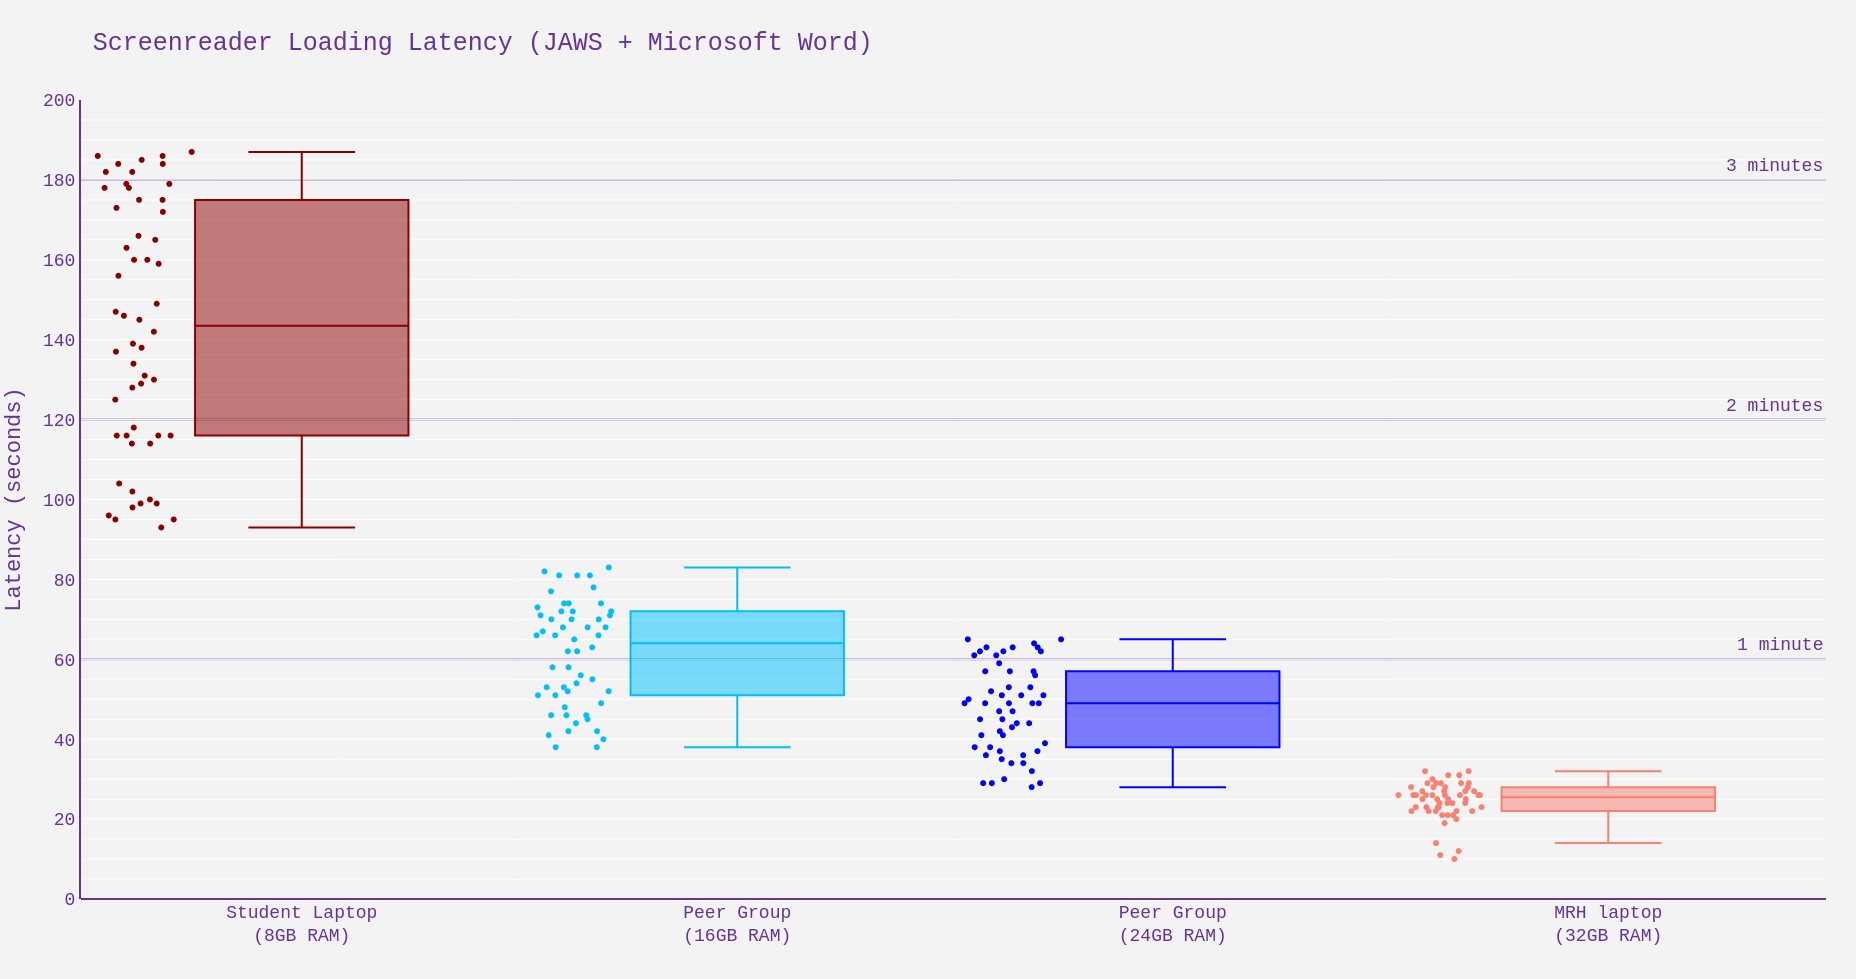
\includegraphics[width=\textwidth]{images/ComputerRBDisplaySpecsTVIFig1.png}
	\caption[Latency to Load JAWS]{Plot showing Latency to Load JAWS while Microsoft Word is open across a student laptop (Dell Latitude 3190 with \textit{8GB RAM}) a high quality student laptop (Dell Precision 3530 with \textit{16GB RAM}), professional laptop (Lenovo ThinkPad E16 with\textit{24 GB RAM}), and a high power laptop (Microsoft Surface Laptop 3 with \textit{32 GB RAM}).}
	\label{fig:figure 1}
\end{figure}

\pagebreak
\pagebreak
\hypertarget{screenreader-response}{%
	\phantomsection\subsection{Screenreader Responsiveness}\label{screenreader-response}}

\begin{longtable}[]{@{}
	>{\raggedright\arraybackslash}m{.4\textwidth}
	>{\raggedright\arraybackslash}m{.25\textwidth}
	>{\raggedright\arraybackslash}m{.25\textwidth}
	@{}
	}

	\toprule\noalign{}

	\textbf{Computer} \break (Color as Labelled in Figure 1)                                                                                                                                        & \textbf{Loading Time}\break (median [Range])                                                                                                               & \textbf{Response Lag}\break (median [Range])
	\\
	\midrule\noalign{}
	\endhead \hline                                                                                                                                                                                                                                                                                                                                                                                                                                                                                                                                                                                                                                                      \\
	\multicolumn{3}{r}{\textbf{Continued on Next Page}} \endfoot
	\endlastfoot
	\fcolorbox{red}{red}{\rule{0pt}{6pt}\rule{6pt}{0pt}}\qquad $\begin{array}{l}\textbf{Students Laptop}\footnote{Dell Latitude 3190} \\ \text{8GB RAM}\end{array}$                                 & 143 [93-183] \footnote{These are the data plotted in Figure 1 above. The responsiveness data are more clear when presented as a table here than as a plot} & 38 [27-91]\footnote{It is further important to note here that any lag in screenreader responsiveness of \textgreater1 sec means the student is behind their peers and their educational opportunity is limited by the technology not being sufficient (\emph{i.e.}, not an adequate accommodation). } \\[1.5em]
	\fcolorbox{cyan}{cyan}{\rule{0pt}{6pt}\rule{6pt}{0pt}}\qquad$\begin{array}{l}\textbf{Student/Professional Laptop}\footnote{Dell Precision 3530} \\ \text{16GB RAM}\end{array}$                  & 64 [38-93]                                                                                                                                                 & 9 [4-15]                                                                                                                                                                                                                                                                                              \\[1.5em]
	\fcolorbox{violet}{violet}{\rule{0pt}{6pt}\rule{6pt}{0pt}}\qquad$\begin{array}{l}\textbf{Professional Laptop}\footnote{Lenovo ThinkPad E16--TVI Personal Laptop} \\ \text{24GB RAM}\end{array}$ & 49 [26-65]                                                                                                                                                 & 1 [0.05-2.5]                                                                                                                                                                                                                                                                                          \\[1.5em]
	\fcolorbox{orange}{orange}{\rule{0pt}{6pt}\rule{6pt}{0pt}}\qquad$\begin{array}{l}\textbf{Professional Laptop}\footnote{Microsoft Surface 3--My Personal Laptop} \\ \text{32GB RAM}\end{array}$  & 25 [10-32]                                                                                                                                                 & 0.5 [0.01-1]\footnote{0.01 is for immediate responses that could not be measured}                                                                                                                                                                                                                     \\ [1.5em] \hline \caption{Lag in JAWS Reporting HTML Content} \\
\end{longtable}

\pagebreak \hypertarget{notes-on-future-proofing-laptops}{%
	\section{Laptop Cost Factors}\label{notes-on-future-proofing-laptops}}
\hypertarget{future-proofing}{%
	\phantomsection\subsection{Laptop Durability}\label{future-proofing}}

I asked ChatGPT why we should consider future usage needs of a laptop into my purchasing plans and here is its response:

\begin{leftbar} \begin{quote}
		Buying laptops with high-end RAM and processor specifications can be beneficial for several reasons, especially in terms of longevity and performance. Here are some key considerations:

		\begin{enumerate}[leftmargin=*]
			\def\labelenumi{\arabic{enumi}.}

			\item
			      Future-Proofing:
		\end{enumerate}

		\begin{itemize}

			\item
			      Investing in higher-end components can help future-proof your laptop to some extent. As software and applications become more demanding over time, a laptop with better specifications is likely to remain relevant and capable of handling new software updates and requirements.
		\end{itemize}

		\begin{enumerate}[leftmargin=*]
			\def\labelenumi{\arabic{enumi}.}
			\setcounter{enumi}{1}

			\item
			      Multitasking and Performance:
		\end{enumerate}

		\begin{itemize}

			\item
			      Higher RAM allows for better multitasking capabilities. If you use resource-intensive applications or run multiple programs simultaneously, having ample RAM prevents slowdowns and ensures smooth performance.
			\item
			      A powerful processor can handle complex computations and tasks more efficiently, contributing to faster overall system performance.
		\end{itemize}

		\begin{enumerate}[leftmargin=*]
			\def\labelenumi{\arabic{enumi}.}
			\setcounter{enumi}{2}

			\item
			      Graphics Processing:
		\end{enumerate}

		\begin{itemize}

			\item
			      For tasks such as video editing, gaming, or other graphics-intensive applications, a high-end GPU (Graphics Processing Unit) is crucial. This is separate from RAM and the main processor but is equally important for certain tasks.
		\end{itemize}

		\begin{enumerate}[leftmargin=*]
			\def\labelenumi{\arabic{enumi}.}
			\setcounter{enumi}{3}

			\item
			      Long-Term Usability:
		\end{enumerate}

		\begin{itemize}

			\item
			      Technology advances quickly, and what is considered high-end today might become standard or entry-level in a few years. However, starting with a high-end laptop gives you a more extended period before your system becomes outdated.
		\end{itemize}

		\begin{enumerate}[leftmargin=*]
			\def\labelenumi{\arabic{enumi}.}
			\setcounter{enumi}{4}

			\item
			      Smooth Upgrades:
		\end{enumerate}

		\begin{itemize}

			\item
			      Some laptops allow users to upgrade certain components like RAM and storage. Starting with higher-end specifications provides more headroom for future upgrades, allowing you to extend the useful life of your laptop.
		\end{itemize}

		\begin{enumerate}[leftmargin=*]
			\def\labelenumi{\arabic{enumi}.}
			\setcounter{enumi}{5}

			\item
			      Resource-Intensive Applications:
		\end{enumerate}

		\begin{itemize}

			\item
			      If you use applications that require a lot of processing power, like video editing software, 3D modeling tools, or virtualization software, a high-end laptop can handle these tasks more efficiently, providing a better user experience.
		\end{itemize}

		\begin{enumerate}[leftmargin=*]
			\def\labelenumi{\arabic{enumi}.}
			\setcounter{enumi}{6}

			\item
			      Responsiveness and Speed:
		\end{enumerate}

		\begin{itemize}

			\item
			      A faster processor and more RAM contribute to a more responsive system. Applications load quicker, and the overall user experience is smoother, which can significantly impact productivity.
		\end{itemize}

		\begin{enumerate}[leftmargin=*]
			\def\labelenumi{\arabic{enumi}.}
			\setcounter{enumi}{7}

			\item
			      Enhanced Resale Value:
		\end{enumerate}

		\begin{itemize}

			\item
			      High-end laptops generally retain their value better than lower-end models. If you decide to sell or upgrade your laptop in the future, having top-tier specifications can make it more attractive to potential buyers.
		\end{itemize}

		It's important to note that the specific requirements depend on your usage patterns and needs. Not everyone needs the highest specifications, and sometimes a mid-range laptop can be more than sufficient for everyday tasks. However, for users with demanding workloads or those who want a longer usable life from their device, opting for higher-end specifications can be a wise investment.
	\end{quote}\end{leftbar}

Other than the resale value we agree with all of the reasons given. we am a recycle the computer back to the vendor rather than a sell it to someone that doesn't understand the limitations that are leading me to sell the equipment kind of person.

\hypertarget{optimizing-cost-with-performance}{%
	\phantomsection\subsection{Laptop Cost Optimization}\label{optimizing-cost-with-performance}}

There is an economic theory based on a Terry Pratchett novel that explains this phenomenon better than we can. It is called the \href{https://en.wikipedia.org/wiki/Boots_theory}{Boots theory}\footnote{Full Text (emphasis mine):
	\begin{leftbar} \begin{quote}The reason that the rich were so rich, Vimes reasoned, was because they managed to spend less money.

			Take boots, for example. He earned thirty-eight dollars a month plus allowances. A really good pair of leather boots cost fifty dollars. But an affordable pair of boots, which were sort of OK for a season or two and then leaked like hell when the cardboard gave out, cost about ten dollars. Those were the kind of boots Vimes always bought, and wore until the soles were so thin that he could tell where he was in Ankh-Morpork on a foggy night by the feel of the cobbles.

			But the thing was that good boots lasted for years and years. \textbf{A man who could afford fifty dollars had a pair of boots that’d still be keeping his feet dry in ten years’ time, while the poor man who could only afford cheap boots would have spent a hundred dollars on boots in the same time and would still have wet feet.}

			Basically, \textbf{we are destined to be stuck in a cycle of perpetually spending more money for inferior products and will, in the end, spend more money than if we just paid for better product in the first place.} -- \textit{Men At Arms}, page 38
		\end{quote}\end{leftbar}  }

\hfill \break The table below illustrates this theory in terms of student laptop computers (Assuming student has a laptop using a screenreader through 3rd-12th grade).

I put this Table here to illustrate why we choose to err on the side of spending \$2000-3000 now on a laptop that will last 3-5 years over spending \$1500-2000 on a laptop that will barely make it 1-2 years before becoming obsolete. By the end of 5 years we will have spent more on Low End and Mid Range Laptops than we would have had we purchased a High End Laptop. Importantly; however, we also would have been using laptops that always perform more poorly than a High End laptop would.

\hspace{-1cm} \begin{longtable}[]{@{}
	>{\raggedright\arraybackslash}m{.15\textwidth}
	>{\raggedright\arraybackslash}m{.05\textwidth}
	>{\raggedright\arraybackslash}m{.05\textwidth}
	>{\raggedright\arraybackslash}m{.05\textwidth}
	>{\raggedright\arraybackslash}m{.05\textwidth}
	>{\raggedright\arraybackslash}m{.05\textwidth}
	>{\raggedright\arraybackslash}m{.05\textwidth}
	>{\raggedright\arraybackslash}m{.05\textwidth}
	>{\raggedright\arraybackslash}m{.05\textwidth}
	>{\raggedright\arraybackslash}m{.05\textwidth}
	>{\raggedright\arraybackslash}m{.05\textwidth}
	>{\raggedright\arraybackslash}m{.10\textwidth}@{}
	}
	\toprule\noalign{}
	                                                                                                                                                                                       &
	\multicolumn{10}{c}{\textbf{Does School Have to Purchase a Replacement Laptop by Year}}                                                                                                &                                                                                                                                                                           \\
	\cline{2-11}                                                                                                                                                                                                                                                                                                                                                       \\
	\textbf{RAM} \break \textbf{Cost}                                                                                                                                                      & \textbf{1}   & \textbf{2}   & \textbf{3}   & \textbf{4}   & \textbf{5}   & \textbf{6}   & \textbf{7}   & \textbf{8}   & \textbf{9}   & \textbf{10}  & \textbf{Total Cost} \\
	\midrule\noalign{}
	\endhead \hline                                                                                                                                                                                                                                                                                                                                                    \\
	\multicolumn{6}{r}{\textbf{Continued on Next Page}} \endfoot
	\endlastfoot
	\textbf{4GB}\footnote{Dell Latitude 3190 Education}\footnote{The 4GB Laptop cannot run JAWS and is only included here to show a price comparison to the other options} \break \$525.04 & $\checkmark$ & $\checkmark$ & $\checkmark$ & $\checkmark$ & $\checkmark$ & $\checkmark$ & $\checkmark$ & $\checkmark$ & $\checkmark$ & $\checkmark$ & \$5,250             \\[1.5em]
	\textbf{8GB} \break \$1184\footnote{Dell Latitude 3190 Education}                                                                                                                      & $\checkmark$ & $\checkmark$ & $\checkmark$ & $\checkmark$ & $\checkmark$ & $\checkmark$ & $\checkmark$ & $\checkmark$ & $\checkmark$ & $\checkmark$ & \$11,840            \\[1.5em]
	\textbf{16GB} \break \$1751\footnote{Dell Precision 3530 given to TVIs teaching screenreaders}                                                                                         & $\checkmark$ & --           & $\checkmark$ & --           & $\checkmark$ & --           & $\checkmark$ & --           & $\checkmark$ & --           & \$8,755             \\[1.5em]
	\hdashline[0.5pt/5pt]                                                                                                                                                                                                                                                                                                                                              \\
	\textbf{32GB}\break \$2824\footnote{Microsoft Surface Laptop 3}\break \textcolor{red}{Best Case}\footnote{This is my personal experience}                                              & $\checkmark$ & --           & --           & --           & --           & $\checkmark$ & --           & --           & --           & --           & \$5,648             \\[1.5em] \\

	\textbf{32GB}\break \$2824\footnote{Microsoft Surface Laptop 3}\break \textcolor{red}{Cautious}                                                                                        & $\checkmark$ & --           & --           & $\checkmark$ & --           & --           & $\checkmark$ & --           & --           & --           & \$8,472             \\[1.5em] \hline


	\caption[Cost of Laptops over Time]{Cost of Laptops Across Time. Notice that the final cost of the 32GB option is comparable to the 4GB over 10 years. However, the 4GB laptop is not capable of running JAWS reliably in the classroom setting.
		\begin{itemize}
			\item For the Best Case Scenario, the 32GB laptop is between \$3,107 and \$6,192 \textit{\textbf{cheaper}} over time compared to the 16 GB and 8GB laptops, respectively.
			\item For the Cautious Scenario, the 32GB laptop is between \$283 and \$3,386 \textit{\textbf{cheaper}} over time compared to the 16 GB and 8GB laptops, respectively.
		\end{itemize}}
\end{longtable}

\pagebreak \hypertarget{minimum-laptop-recommendations}{%
	\section{Recommended Laptop Specifications}\label{minimum-laptop-recommendations}}

\begin{longtable}[]{@{}
	>{\raggedright\arraybackslash}m{.5\textwidth}
	>{\raggedright\arraybackslash}m{.5\textwidth}@{}
	}
	\toprule\noalign{}

	\textbf{Use Case}                             & \textbf{Recommendation} \\
	\midrule\noalign{}
	\endhead \hline                                                         \\
	\multicolumn{2}{r}{\textbf{Continued on Next Page}} \endfoot
	\endlastfoot
	\multicolumn{2}{l}{\textbf{Screenreader Only}}                          \\
	\break JAWS Screenreader                      & \textbf{24-32GB}        \\[2em]
	\break NVDA Screenreader                      & \textbf{24-32GB}        \\[2em]
	\break Dolphin Screenreader                   & \textbf{24-32GB}        \\[2em]
	\break ZDSR Screenreader                      & \textbf{24-32GB}        \\[2em]
	\multicolumn{2}{l}{\textbf{Screenreader + Magnification}}               \\
	\break JAWS Screenreader + Windows Magnifier  & \textbf{24-32GB}        \\[2em]
	\break NVDA Screenreader + Windows Magnifier  & \textbf{24-32GB}        \\[2em]
	\break SuperNova Screenreader + Magnification & \textbf{32-64GB}        \\[2em]
	\break Fusion Screenreader + Magnification    & \textbf{32-64GB}        \\[2em] \hline
	\caption{Recommended Laptop Specifications}
\end{longtable}

\pagebreak
\hypertarget{laptops-meeting-redcommended-specifications}{%
	\section{Laptops Meeting Specifications}\label{laptops-meeting-redcommended-specifications}}

\begin{longtable}[]{@{}
	>{\raggedright\arraybackslash}m{.3\textwidth}
	>{\raggedright\arraybackslash}m{.12\textwidth}
	>{\raggedright\arraybackslash}m{.12\textwidth}
	>{\raggedright\arraybackslash}m{.12\textwidth}
	>{\raggedright\arraybackslash}m{.12\textwidth}
	>{\raggedright\arraybackslash}m{.2\textwidth}@{}
	}
	\toprule\noalign{}

	\textbf{Company / Model}                                                                                    & \textbf{Cost}                             & \textbf{Keyboard}      & \textbf{RAM} & \textbf{Screen Size} & \textbf{Processor} \\
	\midrule\noalign{}
	\endhead \hline                                                                                                                                                                                                                             \\
	\multicolumn{6}{r}{\textbf{Continued on Next Page}} \endfoot
	\endlastfoot
	Framework 13                                                                                                & \$1,102                                   & QWERTY                 & 32GB         & 13.5''               & 13th Gen i7        \\[1.5em]
	Framework 13                                                                                                & \$2,222                                   & QWERTY                 & 64GB         & 13.5''               & 13th Gen i7        \\[1.5em]
	Framework 13                                                                                                & \$1,732                                   & QWERTY                 & 32GB         & 13.5''               & AMD Ryzen 7        \\[1.5em]
	Framework 13                                                                                                & \$1,892                                   & QWERTY                 & 64GB         & 13.5''               & AMD Ryzen 7        \\[1.5em]
	Framework 16                                                                                                & \$2,239                                   & QWERTY\break (+NUMPAD) & 32GB         & 16.0''               & AMD Ryzen 9        \\[1.5em]
	Framework 16\break (+ AMD GPU)                                                                              & \$2,639                                   & QWERTY\break (+NUMPAD) & 32GB         & 16.0''               & AMD Ryzen 9        \\[1.5em]
	Framework 16                                                                                                & \$2,399                                   & QWERTY\break (+NUMPAD) & 64GB         & 16.0''               & AMD Ryzen 9        \\[1.5em]
	Framework 16\break (+ AMD GPU)                                                                              & \$2,799                                   & QWERTY\break (+NUMPAD) & 64GB         & 16.0''               & AMD Ryzen 9        \\[1.5em]
	Dell Precision 5770                                                                                         & \$2,789                                   & QWERTY                 & 32GB         & 17''                 & 12th Gen i7        \\[1.5em]
	Dell XPS 15                                                                                                 & \$2,099                                   & QWERTY                 & 32GB         & 15.6''               & 12th Gen i7        \\[1.5em]
	Dell XPS 15                                                                                                 & \$2,349                                   & QWERTY                 & 32GB         & 15.6''               & 12th Gen i9        \\[1.5em]
	Dell XPS 15                                                                                                 & \$2,999                                   & QWERTY                 & 32GB         & 15.6''               & 13th Gen i9        \\[1.5em]
	Dell XPS 17                                                                                                 & \$3,349                                   & QWERTY                 & 32GB         & 15.6''               & 13th Gen i7        \\[1.5em]
	Dell XPS 17                                                                                                 & \$3,549                                   & QWERTY                 & 32GB         & 15.6''               & 13th Gen i9        \\[1.5em]
	Alienware m16                                                                                 & \$3,499                                   & QWERTY                 & 32GB         & 16.0''               & 13th Gen 19        \\[1.5em]
	Alienware x14                                                                                 & \$1,999                                   & QWERTY                 & 32GB         & 14.0''               & 13th Gen i7        \\[1.5em]
	Dell XPS 13 Plus                                                                                            & \$2,009                                   & QWERTY                 & 32GB         & 13.4''               & 13th Gen i7        \\[1.5em]
	Dell latitude 7440                                                                                          & \$3,615                                   & QWERTY                 & 32GB         & 14.0''               & 13th Gen i7        \\[1.5em]
	Dell G16 Gaming Laptop                                                                                      & \$1,999                                   & QWERTY                 & 32GB         & 16.0''               & 13th Gen i7        \\[1.5em]
	Dell precision 5680                                                                                         & \$5,597                                   & QWERTY                 & 32GB         & 16.0''               & 13th Gen i9        \\[1.5em]
	Dell Inspiron 16 Plus                                                                                       & \$1,499                                   & QWERTY                 & 32GB         & 16.0''               & 13th Gen i7        \\[1.5em]
	Dell precision 7680                                                                                         & \$7,225                                   & QWERTY                 & 32GB         & 16.0''               & 13th Gen i9        \\[1.5em]
	Dell Precision 5480                                                                                         & \$4,354                                   & QWERTY                 & 32GB         & 14.0''               & 13th Gen i7        \\[1.5em]
	Dell Precision 3480                                                                                         & \$3,205                                   & QWERTY                 & 32GB         & 14.0''               & 13th Gen i7        \\[1.5em]
	Dell Precision 3581                                                                                         & \$3,854                                   & QWERTY                 & 32GB         & 15.6''               & 13th Gen i7        \\[1.5em]
	HP Dragonfly Pro                                                                                            & \$1,549                                   & QWERTY                 & 32GB         & 14.0''               & AMD Ryzen 7        \\[1.5em]
	HP Envy                                                                                                     & \$1,749                                   & QWERTY                 & 32GB         & 17.3''               & 13th Gen i7        \\[1.5em]
	Acer Predator Helios 16                                                                                     & \$2,499                                   & QWERTY                 & 32GB         & 16.0''               & 13th Gen i9        \\[1.5em]
	Acer Predator Triton                                                                                        & \$3,799                                   & QWERTY                 & 64GB         & 17.0''               & 13th Gen i9        \\[1.5em]
	Asus ProArt Studiobook                                                                                      & \$2,999                                   & QWERTY                 & 32GB         & 16.0''               & 13th Gen i9        \\[1.5em]
	Asus Zenbook Pro 16X                                                                                        & \$2,599                                   & QWERTY                 & 32GB         & 16.0''               & 13th Gen i9        \\[1.5em]
	MSI Vector                                                                                                  & \$1,999                                   & QWERTY                 & 64GB         & 14.0''               & 13th Gen i9        \\[1.5em]
	Lenovo Thinkpad P14s                                                                                        & \$2,509                                   & QWERTY                 & 64GB         & 14.0''               & AND Ryzen 7        \\[1.5em]
	Lenovo Thinkpad P14s                                                                                        & \$2,199                                   & QWERTY                 & 32GB         & 14.0''               & AND Ryzen 7        \\[1.5em]
	Legion Pro 7i                                                                                               & \$3,599                                   & QWERTY                 & 32GB         & 16.0''               & 13th Gen i9        \\[1.5em]
	Lenovo Thinkpad X1 Yoga                                                                                     & \$3,719                                   & QWERTY                 & 32GB         & 14.0''               & 13th Gen i7        \\[1.5em]
	Lenovo ThinkPad P16v                                                                                        & \$3,339                                   & QWERTY                 & 32GB         & 16.0''               & 13th Gen i7        \\[1.5em]
	Lenovo ThinkPad P16v                                                                                        & \$4,929                                   & QWERTY                 & 64GB         & 16.0''               & 13th Gen i7        \\[1.5em]
	Lenovo ThinkPad P16 Gen 2                                                                                   & \$3,239                                   & QWERTY                 & 32GB         & 16.0''               & 13th Gen i7        \\[1.5em]
	Lenovo ThinkPad P16 Gen 2                                                                                   & \$4,189                                   & QWERTY                 & 64GB         & 16.0''               & 13th Gen i7        \\[1.5em]
	Lenovo ThinkPad P16 Gen 2                                                                                   & \$4,829                                   & QWERTY                 & 64GB         & 16.0''               & 13th Gen i7        \\[1.5em]
	Lenovo ThinkPad P16 Gen 2                                                                                   & \$2,039                                   & QWERTY                 & 32GB         & 16.0''               & AMD Ryzen 7        \\[1.5em]
	Lenovo ThinkPad P16 Gen 2                                                                                   & \$2,829                                   & QWERTY                 & 64GB         & 16.0''               & AMD Ryzen 7        \\[1.5em]
	Microsoft Surface Laptop 5                                                                                  & \$2824                                    & QWERTY                 & 32GB         & 15.0''               & 12th Gen i7        \\[1.5em]
	Notey the Notetaker                                                                                         & \textasciitilde\$750+\footnote{Self build
	\href{https://notey-project.com/2023/03/07/notey-user-manual-v1-0-2/}{Specs for Notey the NoteTaker}}       & QWERTY \break Perkins                     & 8GB-16GB               & none         & Celeron
	N5105                                                                                                                                                                                                                                       \\ [1.5em]
	Seika Studio\footnote{This is a Windows Computer without a monitor, substituting a 40 cell braille display} & \$6,500                                   & QWERTY                 & 8GB-16GB     & none                 & 12th Gen i7        \\ [1.5em]
	Orbit Optima\footnote{This is a Windows Computer without a monitor, substituting a 40 cell braille display} & \$6,500                                   & QWERTY                 & 32GB-64GB    & none                 & 13th Gen i7        \\ [1.5em] \hline
	\caption{Laptop Computers Meeting Recommended Specifications}
\end{longtable}

\pagebreak \hypertarget{ios-devices}{%
	\chapter{Transformative Tablets: Pioneering Success for Visually Impaired Students Through Innovative Apps}\label{ios-devices}}
\extramarks{Vision Department Technology Needs}{Transformative Tablets}
In an era where technology shapes the landscape of education, tablets have emerged as transformative tools, providing visually impaired students with unprecedented access to knowledge and fostering independence in their academic journeys. Within the realm of tablets, both iPad and Android devices stand as beacons of innovation, offering not only user-friendly interfaces but also a diverse array of applications specifically tailored to bridge the accessibility gap. This chapter embarks on a compelling exploration of how tablets, in tandem with purpose-built apps, are not just tools but catalysts for success in the educational odyssey of visually impaired students.

The tactile elegance of tablets goes beyond mere convenience; it represents a paradigm shift in the way students interact with information. For visually impaired learners, tablets serve as dynamic portals, offering a multi-sensory approach to engagement. Through the lens of this chapter, we will unravel the unique functionalities of both iPad and Android tablets, delving into their respective strengths and contributions to an inclusive educational experience.

Apps, the lifeblood of these devices, play an instrumental role in transforming tablets into personalized learning companions. From screen readers that convert text to speech with remarkable precision to magnification apps that enhance visual content, the ecosystem of applications available empowers visually impaired students to navigate the digital realm with confidence. This chapter seeks to illuminate how these apps, carefully designed to meet diverse educational needs, not only level the playing field but also pave the way for enhanced participation and academic achievement. Tablets, coupled with innovative apps, are not mere gadgets; they represent a dynamic force propelling visually impaired students toward success. Through this exploration, we aim to underscore the indispensable role these tools play in shaping an educational landscape where every student, regardless of visual abilities, can seize the opportunities that lie ahead.

\hypertarget{tablet-considerations}{%
	\section{Tablet Considerations}\label{tablet-considerations}}
When selecting a tablet for students with visual impairments to access their schoolwork, careful consideration must be given to the device's accessibility features to ensure an inclusive and conducive learning environment. Essential considerations include the tablet's compatibility with screen readers and magnification tools, ensuring that these assistive technologies seamlessly integrate with the device's operating system. Additionally, evaluating the availability and effectiveness of built-in accessibility features such as VoiceOver for iOS or TalkBack for Android is crucial\footnote{Traditionally, assistive technology for the blind has focused on the iPad line since the Android line had historically lagged behind the Apple products for accessibility features prior to 2020 so accessibility apps have favored the iOS/iPadOS architecture. However, groups are emerging that specifically instruct users of Android devices how to access and use accessibility settings \textit{cf.}, \href{Blind Android Users}{https://www.youtube.com/channel/UCvEM-SmpwElNALldhp8hG1g}}. The tablet's tactile features, size, and weight should also be taken into account to accommodate students' specific needs. High contrast and customizable color settings, as well as text-to-speech functionalities, are vital components that enhance readability. Furthermore, the tablet's compatibility with a variety of educational apps designed with accessibility in mind is paramount. By prioritizing these considerations, educators and administrators can empower students with visual impairments to engage with their schoolwork independently and efficiently, fostering a more inclusive learning experience.

One frequently overlooked challenge in using tablets for individuals with visual impairments is the potential for visual fatigue. Recent research, such as the study by Pakdee and Sengsoon (2021) \footnote{\textit{cf}., \href{https://www.researchgate.net/publication/352764109_Immediate_Effects_of_Different_Screen_Sizes_on_Visual_Fatigue_in_Video_Display_Terminal_Users}{Pakdee, S., \& Sengsoon, P. (2021). Immediate Effects of Different Screen Sizes on Visual Fatigue in Video Display Terminal Users. \textit{Iranian Rehabilitation Journal, 19(2)}, 137-1461. DOI:10.32598/irj.19.2.1108.2}}, reveals that opting for a slightly larger device can mitigate visual fatigue, particularly for those engaged in visually demanding tasks. This consideration becomes even more pertinent for individuals with visual impairments.

While the iPad Pro2 and Samsung Galaxy Tab 9 tablets are often lauded for their increased brightness, it's crucial not to prioritize brightness as a major factor. Research suggests that boosting brightness can exacerbate visual fatigue. Instead, emphasis should be placed on the larger screen's enhanced resolution and expanded visual area, facilitating efficient use of Zoom functions. This becomes especially significant when aiming to teach students to adeptly navigate assistive technology without relying solely on pinch zooming, a feature that may not consistently function within all applications.

Another critical consideration involves contrast ratios. For students with photophobia, adjusting luminance levels to lower settings can significantly enhance clarity of text and images. This nuanced approach to tablet selection is pivotal in creating an accessible and comfortable learning environment for students with visual impairments.

\hypertarget{tablet-options}{%
	\section{Tablet Options}\label{tablet-options}}

\begin{longtable}[]{@{}
	>{\raggedright\arraybackslash}m{.3\textwidth}
	>{\raggedright\arraybackslash}m{.1\textwidth}
	>{\raggedright\arraybackslash}m{.1\textwidth}
	>{\raggedright\arraybackslash}m{.2\textwidth}@{}
	>{\raggedright\arraybackslash}m{.3\textwidth}@{}
	}
	\toprule\noalign{}

	\textbf{Tablet}             & \textbf{Cost} & \textbf{Screen}                                                                                                                                                                                                                        & \textbf{Contrast Ratio}                                                                                                                                                                                                                    & \textbf{Features} \\
	\midrule\noalign{}
	\endhead \hline                                                                                                                                                                                                                                                                                                                                                                                                                                                                                                                                       \\
	\multicolumn{3}{r}{\textbf{Continued on Next Page}} \endfoot
	\endlastfoot
	iPad                        & \$599         & 10.9''                                                                                                                                                                                                                                 & 1,417:1                                                                                                                                                                                                                                                        \\[1.5em]
	iPad Air                    & \$749         & 10.9''                                                                                                                                                                                                                                 & 1,417:1                                                                                                                                                                                                                                                        \\[1.5em]
	iPad Pro                    & \$1,099       & 12.9''\footnote{The larger size of the iPad Pro2 screen provides students with access to using Zoom functions that allow student to use the Window Zoom function to magnify portions of the screen while maintaining the overall view} & 1,000,000:1\footnote{The higher contrast ratio allows students to pinch-zoom material to a larger overall size prior to having the material pixelate or blur (note, using the Zoom function re-flows fonts and prevents blurring of fonts}                     \\
	Amazon Fire Max 11          & \$150         & 10.1''                                                                                                                                                                                                                                 &                                                                                                                                                                                                                                            &                   \\
	Samsung Galaxy Tab S9       & \$799         & 11''                                                                                                                                                                                                                                   &                                                                                                                                                                                                                                            &                   \\
	Samsung Galaxy Tab S9 Plus  & \$999         & 11''                                                                                                                                                                                                                                   &                                                                                                                                                                                                                                            &                   \\
	Samsung Galaxy Tab S9 Ultra & \$1,099       & 12.4''                                                                                                                                                                                                                                 &                                                                                                                                                                                                                                            &                   \\
	OnePlus Pad                 & \$480         & 11.6''                                                                                                                                                                                                                                 &                                                                                                                                                                                                                                            &                   \\
	Microsoft Surface Go 3      & \$450         & 10.5''                                                                                                                                                                                                                                 &                                                                                                                                                                                                                                            &                   \\
	Google Pixel Tablet         & \$499         & 10.95''                                                                                                                                                                                                                                &                                                                                                                                                                                                                                            &                   \\
	Lenovo Yoga Tab 13          & \$1,165       & 13''                                                                                                                                                                                                                                   &                                                                                                                                                                                                                                            &                   \\
	Placeholder                 & x             & x                                                                                                                                                                                                                                      & x                                                                                                                                                                                                                                          & x                 \\[1.5em]\hline
	\caption[Recommended Tablet Specifications]{Recommended Tablet Specifications}
\end{longtable}


\pagebreak \hypertarget{tablet-apps}{%
	\section{Mobile Applications}\label{tablet-apps}}

\begin{longtable}[]{@{}
	>{\raggedright\arraybackslash}m{.3\textwidth}
        >{\raggedright\arraybackslash}m{.1\textwidth}
	>{\raggedright\arraybackslash}m{.3\textwidth}@{}
 	>{\raggedright\arraybackslash}m{.3\textwidth}@{}
	}
	\toprule\noalign{}

	\textbf{App}  & \textbf{Cost} & \textbf{Function} & \textbf{OS}\\
	\midrule\noalign{}
	\endhead \hline \\
\multicolumn{3}{r}{\textbf{Continued on Next Page}} \endfoot
	\endlastfoot
\multicolumn{4}{l}{\textbf{Accessibility Training}}\\[1em]
Ballyland Rotor & \$2.99 & Train VoiceOver rotor & iOS/iPadOS \\[1.5em]
Ballyland Magic Plus & \$3.99 & Train VoiceOver Gestures & iOS/iPadOS\\[1.5em]
VO Lab & \$4.99 & Train VoiceOver Gestures\break (meant for adolescents) & iOS/iPadOS \\[1.5em]
\multicolumn{4}{l}{\textbf{Cortical Vision Impairment}}\\[1em]
Sensory Light Box & free & Gaze training & iOS/iPadOS \\[1.5em]
CVI Connect Pro & free & CVI-based Vision Training & OS \\[1.5em]
\multicolumn{4}{l}{\textbf{Audiobook/Reading}}\\[1em]
Dolphin EZ Reader & free & DAISY Reader & iOS/iPadOS\break AndroidOS 13+\\[1.5em]
VoiceDream Reader & free\footnote{requires \$79.99/yr subscription and additional \$4.99 for each premium voice} & DAISY Reader & iOS/iPadOS\\[1.5em]
Bookshare Reader  & free & DAISY Reader & iOS/iPadOS\\[1.5em]
Kindle & free\footnote{requires books to be purchased} & e-Book & iOS/iPadOS\break AndroidOS 13+\\[1.5em]
Libby & free\footnote{requires a library membership}   & Audiobook & iOS/iPadOS\break AndroidOS 13+\\[1.5em]
Audible& free\footnote{requires books to be purchased} & Audiobook\ & iOS/iPadOS\break AndroidOS 13+\\[1.5em]
BARD Mobile & free\footnote{requires account with local affiliate State Library for the Blind} & e-Book & iOS/iPadOS\break AndroidOS 13+\\[1.5em]
KNFB Reader\break(rebranded OneStepReader) & \$99.99   & OCR/Reading & iOS/iPadOS\break AndroidOS 13+ \\[1.5em]
Audible& free\footnote{requires books to be purchased} & Audiobook & iOS/iPadOS\break AndroidOS 13+\\[1.5em]
\multicolumn{4}{l}{\textbf{Productivity/Schoolwork}}\\[1em]
Notability &free\footnote{with in app puchases} & Scan \& Markup Documents & iOS/iPadOS \break AndroidOS 13+\\[1.5em]
GoodNotes  &free\footnote{with in app puchases}  & Scan \& Markup Documents & iOS/iPadOS \break AndroidOS 13+\\[1.5em]
My Board Buddy  & free & all the things  & iOS/iPadOS\\[1.5em]
Desmos Graphing Calculator & free & all the things  & iOS/iPadOS \break AndroidOS 13+\\[1.5em]
Desmos Scientific Calculator & free & all the things  & iOS/iPadOS \break AndroidOS 13+\\[1.5em]
\multicolumn{4}{l}{\textbf{Optical Character Recognition}}\\[1em]
KNFB Reader\break(rebranded OneStepReader) & \$99.99   & OCR/Reading & iOS/iPadOS\break AndroidOS 13+ \\[1.5em]
SeeingAI & free & talking camera\break OCR & iOS/iPadOS\break AndroidOS 13+ \\[1.5em]
TapTapSee & free & talking camera\break OCR & iOS/iPadOS\break AndroidOS 13+ \\[1.5em]
\multicolumn{4}{l}{\textbf{Orientation \& Mobility / Navigation}} \\[1em]
HapticNav         & free\footnote{requires in app puchases} & Haptic turn by turn GPS navigation  & iOS/iPadOS\break AndroidOS 13+      \\[1.5em]
BlindSquare       & \$39.99                 &       & iOS/iPadOS     \\[1.5em]
XploreNinja       & \$39.99  & MIPSoft & AndroidOS 13+\\[1.5em]
WeWalk            & free\footnote{requires in app puchases} &        & iOS/iPadOS     \\[1.5em]
Google Maps       & free                    &  Turn by Turn GPS Navigation    & iOS/iPadOS\break AndroidOS 13+     \\[1.5em]
Apple Maps        & free                    &  Turn by Turn GPS Navigation       & iOS/iPadOS       \\[1.5em]
Moovit            & free\footnote{requires in app puchases} &  Local Public Transit      & iOS/iPadOS\break AndroidOS 13+      \\[1.5em]
Waymap            & free                    &  Turn by Turn GPS Navigation\break Focuses on indoor navigation    & iOS/iPadOS\break AndroidOS 13+       \\[1.5em]
Seeing Eye GPS    & free\footnote{requires in app puchases} & Turn by Turn GPS Navigation   & iOS/iPadOS\break AndroidOS 13+      \\[1.5em]\hline
	\caption[Mobile/Tablet Apps]{Mobile/Tablet Apps}
\end{longtable}

\pagebreak \hypertarget{braille-first-devices}{%
	\chapter{Bridging Literacy: The Crucial Role of Refreshable Braille Displays in Empowering Visually Impaired Students}\label{braille-first-devices}}
\extramarks{Vision Department Technology Needs}{Bridging Literacy}
In the intricate tapestry of education, the pursuit of literacy is a fundamental thread, weaving through the academic journey of every student. For visually impaired learners, the path to literacy takes on a unique character, one in which the tactile elegance of braille becomes a vital conduit to knowledge. Within this narrative, refreshable braille displays emerge as indispensable companions, unlocking the doors to literacy, fostering engagement, and propelling students toward academic success. This chapter embarks on a compelling exploration of how refreshable braille displays are not merely tools but keystones in the quest for literacy and educational achievement among visually impaired students.

At the heart of this exploration lies the transformative power of refreshable braille displays—a technological marvel that seamlessly integrates the tactile richness of braille with the dynamic capabilities of digital communication. This chapter delves into the ergonomic design and sophisticated functionalities of these devices, spotlighting their pivotal role in ensuring that visually impaired students not only read but actively participate in the discourse of knowledge acquisition.

Refreshable braille displays play a dual role in the educational narrative of visually impaired students. Firstly, they serve as conduits for accessing textual content, enabling the exploration of literature, textbooks, and diverse educational materials in a format that aligns with the tactile language of braille. Secondly, and perhaps more profoundly, these devices empower students to actively contribute to the discourse, facilitating note-taking, writing, and engaging in classroom discussions with the same spontaneity and fluency as their sighted peers.

By providing visually impaired students with the means to interact with written information independently and dynamically, these devices emerge not just as tools but as instruments of empowerment, fostering a sense of agency and paving the way for academic success in the rich landscape of education.

\hypertarget{braille-notetakers-and-braille-laptop-computers}{%
	\section{Braille Notetakers and Laptops}\label{braille-notetakers-and-braille-laptop-computers}}

\begin{longtable}[]{@{}
	>{\raggedright\arraybackslash}m{.25\textwidth}
	>{\raggedright\arraybackslash}m{.15\textwidth}
	>{\raggedright\arraybackslash}m{.15\textwidth}
	>{\raggedright\arraybackslash}m{.15\textwidth}
	>{\raggedright\arraybackslash}m{.15\textwidth}
	>{\raggedright\arraybackslash}m{.15\textwidth}@{}
	}
	\toprule\noalign{}

	\textbf{Display}                                                                                                                                                                                                                             & \textbf{Cost}                                                                                                             & \textbf{Battery} & \textbf{Keyboard} & \textbf{Manufacturer} & \textbf{OS}                                                                                                                                                                                                                                                                                                                                                                                 \\
	\midrule\noalign{}
	\endhead \hline                                                                                                                                                                                                                                                                                                                                                                                                                                                                                                                                                                                                                                                                                                                                                                                                                       \\
	\multicolumn{6}{r}{\textbf{Continued on Next Page}} \endfoot
	\endlastfoot
	Orbit Optima\footnote{This is a Windows Computer without a monitor that runs on any screenreader, but it has settings to function like a braille notetaker}                                                                                  & \$6,000                                                                                                                   & TBD              & QWERTY            & Orbit Research        & Windows 11                                                                                                                                                                                                                                                                                                                                                                                  \\[1.5em]
	ElBraille 40\footnote{This is a Windows Computer without a monitor that runs on JAWS, but it has settings to function like a braille notetaker} \footnote{This is not included above as a laptop option since it has only 4GB of RAM}        & \$6,000\footnote{This price is for the ElBraille unit itself as well as a Focus 40 that docks into the unit as a display} & TBD              & QWERTY            & Elita                 & Windows 10\footnote{Windows 11 is not yet officially supported, but users are updating to Windows 11 without issue}                                                                                                                                                                                                                                                                         \\[1.5em]
	Seika Studio\footnote{This is a Windows Computer without a monitor, but it has settings to function like a braille notetaker}                                                                                                                & \$6,500                                                                                                                   & TBD              & QWERTY            & Nippon Telesoft       & Windows 10                                                                                                                                                                                                                                                                                                                                                                                  \\[1.5em]

	BrailleNote Touch+\footnote{For both the BrailleNote Touch+ and BrailleSense 6, there is an emerging issue with outdated operating systems, WiFi connectivity inconsistencies, and incompatibility with Google applications. \begin{itemize}
			                                                                                                                                                                                                                             \item
			                                                                                                                                                                                                                                   \href{https://perkins.org/braillenote-touch-outdated-os/}{Link to article from Perkins.org regarding the BrailleNote Touch Plus}
			                                                                                                                                                                                                                             \item
			                                                                                                                                                                                                                                   \href{https://endoflife.date/android}{Continually Updated List for End of Life for all flavors of AndroidOS}
		                                                                                                                                                                                                                             \end{itemize}} & \$5,795                                                                                                                   & 12h              & Perkins           & Humanware             & Android 8\footnote{Android 8 `Oreo' Security Support Ended (\emph{i.e.}, End of Life) 2017-12-05}                                                                                                                                                                                                                                                                                            \\[1.5em]
	BrailleSense 6                                                                                                                                                                                                                               & \$5,795                                                                                                                   & 12h              & Perkins           & HIMS                  & Android 10\footnote{Android 10 `Queen Cake' Security Support Ended (\emph{i.e.}, End of Life) 2023-03-06}\footnote{The Braillesense has a firmware update v2.0 released 2023-11-28 which updates the operating system to Android 12, but this is currently buggy and causing system overheating. (\emph{note:} Android 12 will only receive updates until \textasciitilde October of 2024)} \\[1.5em]
	InsideONE                                                                                                                                                                                                                                    & \$5,499                                                                                                                   & 6h               & Perkins           & InsideVision          & Windows 11                                                                                                                                                                                                                                                                                                                                                                                  \\[1.5em]
	Nattiq Note                                                                                                                                                                                                                                  & \$5,200                                                                                                                   & 12h              & QWERTY            & Nattiq                & Windows 11                                                                                                                                                                                                                                                                                                                                                                                  \\[1.5em]
	Notey the Notetaker                                                                                                                                                                                                                          & \textasciitilde\$750+\footnote{Self build
	\href{https://notey-project.com/2023/03/07/notey-user-manual-v1-0-2/}{Specs for Notey the NoteTaker}}                                                                                                                                        &                                                                                                                           & QWERTY Perkins   & Miscs             & Windows 11                                                                                                                                                                                                                                                                                                                                                                                                          \\[1.5em]
	b.note                                                                                                                                                                                                                                       & \$4,360                                                                                                                   & 15h              & Perkins           & Eurobraille           & Proprietary                                                                                                                                                                                                                                                                                                                                                                                 \\[1.5em]\hline
	\caption{ Braille NoteTakers and Laptops }
\end{longtable}
\pagebreak \hypertarget{refreshable-braille-displays}{%
	\section{Refreshable Braille
	  Displays}\label{refreshable-braille-displays}}

\hypertarget{few-cell-refreshable-braille-displays}{%
	\phantomsection\subsection{14-20 cell Refreshable Braille
		Displays}\label{few-cell-refreshable-braille-displays}}

\begin{flushleft} \begin{longtable}[]{@{}
		>{\raggedright\arraybackslash}m{.25\textwidth}
		>{\raggedright\arraybackslash}m{.15\textwidth}
		>{\raggedright\arraybackslash}m{.15\textwidth}
		>{\raggedright\arraybackslash}m{.15\textwidth}
		>{\raggedright\arraybackslash}m{.15\textwidth}@{}
		}
		\toprule\noalign{}

		\textbf{Display}                                                                                             & \textbf{Cost} & \textbf{Battery} & \textbf{Keyboard} & \textbf{Manufacturer} \\
		\midrule\noalign{}
		\endhead \hline                                                                                                                                                                             \\
		\multicolumn{5}{r}{\textbf{Continued on next page}}
		\endfoot	\endlastfoot
		Brailliant BI20x                                                                                             & \$2,199       & 14               & Perkins           & Humanware             \\[1.5em]
		Focus 14 Blue                                                                                                & \$1,545       & 18               & Perkins           & Vispero               \\[1.5em]
		Chameleon 20                                                                                                 & \$1,715       & 14               & Perkins           & APH                   \\[1.5em]
		Orbit Reader 20+                                                                                             & \$799         & 20               & Perkins           & Orbit Research        \\[1.5em]
		Orbit Speak\footnote{This device has no braille output, but uses braille input and returns aauditory output} & TBD           & 20               & Perkins           & Orbit Research        \\[1.5em]
		Actilino                                                                                                     & \$2,795       & 16               & Perkins           & Help Tech             \\[1.5em]
		Basic Braille 20                                                                                             & \$2,295       & 16               & none              & Help Tech             \\[1.5em]
		VarioUltra 20                                                                                                & \$4,340       & 12               & Perkins           & VisioBraille          \\[1.5em]
		Seika Mini Plus                                                                                              & \$2,795       & 20               & none              & Nippon Telesoft       \\[1.5em]
		Seika 24                                                                                                     & \$2,395       & 20               & none              & Nippon Telesoft       \\[1.5em]
		b.note 20                                                                                                    & \$2,695       & 15               & Perkins           & Eurobraille           \\[1.5em] \hline
		\caption[ 14-20 cell Single Line Refreshable Braille Displays -]{ 14-20 cell Single Line Refreshable Braille Displays -}
	\end{longtable}  \end{flushleft}

\pagebreak \hypertarget{cell-refreshable-braille-displays}{%
	\phantomsection\subsection{32-40 cell Refreshable Braille
	  Displays}\label{cell-refreshable-braille-displays}}

\begin{longtable}[]{@{}
	>{\raggedright\arraybackslash}m{.25\textwidth}
	>{\raggedright\arraybackslash}m{.15\textwidth}
	>{\raggedright\arraybackslash}m{.15\textwidth}
	>{\raggedright\arraybackslash}m{.15\textwidth}
	>{\raggedright\arraybackslash}m{.15\textwidth}@{}
	}
	\toprule\noalign{}

	\textbf{Display}   & \textbf{Cost} & \textbf{Battery} & \textbf{Keyboard} & \textbf{Manufacturer} \\
	\midrule\noalign{}
	\endhead \hline                                                                                   \\
	\multicolumn{5}{r}{\textbf{Continued on Next Page}} \endfoot
	\endlastfoot
	Brailliant BI40x   & \$3,195       & 14               & Perkins           & Humanware             \\[1.5em]
	Focus 40 Blue      & \$3,145       & 18               & Perkins           & Vispero               \\[1.5em]
	Mantis Q40         & \$2,495       & 14               & QWERTY            & APH                   \\[1.5em]
	Orbit Reader 40    & \$1,399       & 20               & Perkins           & Orbit Research        \\[1.5em]
	QBraille XL        & \$3,195       & 16               & Perkins           & HIMS                  \\[1.5em]
	Basic Braille Plus & \$3,295       & 12               & Perkins           & Help Tech             \\[1.5em]
	Active Star        & \$6,795       & 40               & Perkins           & Help Tech             \\[1.5em]
	Active Braille     & \$6,495       & 20               & Perkins           & Help Tech             \\[1.5em]
	Activator          & \$6,495       & 40               & Perkins           & Help Tech             \\[1.5em]
	Vario Ultra 40     & \$7,643       & 12               & Perkins           & VisioBraille          \\[1.5em]
	Vario 340          & \$5,138       & 20               & none              & VisioBraille          \\[1.5em]
	Vario 440          & \$4,550       & 20               & none              & VisioBraille          \\[1.5em]
	Seika V5           & \$2,495       & 20               & none              & Nippon Telesoft       \\[1.5em]
	Alva 640 Comfort   & \$3,046       & 10               & Perkins           & Optelec               \\[1.5em]
	Alva 640 USB       & \$3837        & n/a              & none              & Optelec               \\[1.5em]
	Alva BC 640        & \$2,087       & 10               & none              & Alva                  \\[1.5em]
	b.note             & \$3,565       & 15               & Perkins           & Eurobraille           \\[1.5em] \hline
	\caption{ 32-40 cell Single Line Refreshable Braille Displays }
\end{longtable}

\pagebreak \hypertarget{multiple-line-refreshable-braille-displaystablets}{%
	\phantomsection\subsection{Multiple Line Braille Displays/Tablets}\label{multiple-line-refreshable-braille-displaystablets}}

\begin{longtable}[]{@{}
	>{\raggedright\arraybackslash}m{.2\textwidth}
	>{\raggedright\arraybackslash}m{.1\textwidth}
	>{\raggedright\arraybackslash}m{.1\textwidth}
	>{\raggedright\arraybackslash}m{.15\textwidth}
	>{\raggedright\arraybackslash}m{.15\textwidth}
	>{\raggedright\arraybackslash}m{.15\textwidth}@{}
	}
	\toprule\noalign{}

	\textbf{Display} & \textbf{Cost}                      & \textbf{Battery} & \textbf{Braille Lines}                 & \textbf{Keyboard} & \textbf{Manufacturer}              \\
	\midrule\noalign{}
	\endhead \hline                                                                                                                                                            \\
	\multicolumn{6}{r}{\textbf{Continued on Next Page}} \endfoot
	\endlastfoot
	Orbit Slate 520  & \$3,495                            & 20-22            & 5 row x 20 cell                        & Perkins           & Orbit Research                     \\[1.5em]
	Orbit Slate 340  & \$3,995                            & 20-22            & 5 row x 20 cell                        & Perkins           & Orbit Research                     \\[1.5em]
	Graphiti         & \textasciitilde\$15,000            & 20-22            & 60 row x 40 cell                       & Perkins           & Orbit Research                     \\[1.5em]
	Graphiti Plus    & \textasciitilde\$15,000            & 20-22            & 60 row x 40 cell + 40 cell line        & Perkins           & Orbit Research                     \\[1.5em]
	TACTIS Table     & \textasciitilde\$15,000 - \$20,000 & Req AC           & 25 row x 40 cell                       & none              & Tactisplay                         \\[1.5em]
	TACTIS Walk      & \textasciitilde\$7,000             & Req AC           & 10 row x 25 cell                       & none              & Tactisplay                         \\[1.5em]
	TACTIS 100       & \textasciitilde\$5,000             & Req AC           & 4 row x 25 cell                        & none              & Tactisplay                         \\[1.5em]
	Canute 360       & \$2,895                            & Req AC           & 9 row x 40 cell                        & none              & Bristol Braille                    \\[1.5em]
	DotPad           & \textasciitilde\$13,000-\$18,000   & 11 hr            & 10 row x 32 cell + 20 cell line        & Touch interface   & Dot Inc.                           \\[1.5em]
	APH Monarch      & \textasciitilde\$13,000-\$18,000   & 11 hr            & 10 row x 32 cell line                  & Perkins           & Dot Inc.\break Humanware\break APH \\[1.5em]
	Blitab           & \$500                              & TBD              & 14 row x 23 cell                       & Touch Interface   & Blitab                             \\[1.5em]
	Tactile Pro      & TBD                                & TBD              & TBD                                    & Perkins           & PCT                                \\[1.5em]
	NewHaptics (?)   & TBD                                & TBD              & TBD                                    & TBD               & New Haptics                        \\[1.5em]
	InsideONE        & \$5,499                            & 6h               & 128GB                                  & Perkins           & InsideVision                       \\[1.5em]
	BraillePad       & \$4,390                            & ?                & 50 row x 40 cells                      & none              & 4Blind                             \\[1.5em]
	Cadence          & TBD                                & ?                & 6 row x 8 cells stack to 24 x 16       & Perkins           & Tactile Engineering                \\[1.5em]
	Tactonom Pro     & \textasciitilde\$15,000            & Requries AC      & 119 col x 89 lines 10,500 touch points & N/A               & Tactonom                           \\[1.5em]\hline
	\caption{ Multiple Line Refreshable Braille Devices }
\end{longtable}
\pagebreak \hypertarget{learning-tools}{%
	\section{Braille Education Devices}\label{learning-tools}}

\begin{flushleft} \begin{longtable}[]{@{}
		>{\raggedright\arraybackslash}m{.3\textwidth}
		>{\raggedright\arraybackslash}m{.1\textwidth}
		>{\raggedright\arraybackslash}m{.6\textwidth}@{}
		}
		\toprule\noalign{}

		\textbf{Equipment}                                        & \textbf{Cost}                                                         & \textbf{Manufacturer}       \\
		\midrule\noalign{}
		\endhead \hline                                                                                                                                                 \\
		\multicolumn{3}{r}{\textbf{Continued on next page}}
		\endfoot	\endlastfoot

		Polly\footnote{Called ``Annie" outside the Unites States} & \$999                                                                 & APH \break THinkerbell Labs \\[1.5em]
		Taptilo                                                   & \$1,349                                                               & HIMS\break OHFA Tech        \\[1.5em]
		Braille Doodle                                            & \$85                                                                  & Touchpad Pro Fundation      \\[1.5em]
		Braille Teach                                             & \$150                                                                 & Braille Teach               \\[1.5em]
		BrailleCoach                                              & \$1,095                                                               & Logan Tech                  \\[1.5em]
		Read Read                                                 & \$645                                                                 & T-var EdVar Tech            \\[1.5em]
		Feelif Pro                                                & \$3,595                                                               & Feelif Technology           \\[1.5em]
		Feelif Creator                                            & \$2,200                                                               & Feelif Technology           \\[1.5em]
		BrailleBlox                                               & \$85 \footnote{Req LeapFrog Fridge Phonics base, \textasciitilde\$20} & BrailleBot                  \\[1.5em]
		BrailleBuzz                                               & \$99                                                                  & APH                         \\[1.5em]
		Mountbatten Braille Tutor                                 & \$5,495                                                               & Harpo                       \\[1.5em]
		SMART Brailler                                            & \$2,195                                                               & Perkins                     \\[1.5em]\hline
		\caption[Braille Education Device]{Braille Education Device}
	\end{longtable}  \end{flushleft}
 
\pagebreak \hypertarget{generation}{%
	\chapter{Empowering Minds: The Crucial Role of High-Quality Braille Embossers in Unlocking STEM Literacy for Visually Impaired Students}\label{generation}}
\extramarks{Vision Department Technology Needs}{Empowering Minds}
In the ever-evolving realms of Science, Technology, Engineering, and Mathematics (STEM), the pursuit of literacy takes on a particularly intricate form. For visually impaired students, the challenges are multifaceted, but with the advent of high-quality braille embossers, a transformative bridge has been constructed. This chapter embarks on a profound exploration of the indispensable role that high-quality braille embossers play in shaping the educational narrative of visually impaired students, especially in the critical domains of Math and STEM. These sophisticated devices, with their ability to translate complex symbols and notations into tangible braille and tactile graphics, stand as pioneers in fostering literacy, comprehension, and success in STEM fields.

The crux of this exploration lies in recognizing the nuanced requirements of visually impaired students pursuing education in Math and STEM disciplines. Traditional print materials, laden with intricate diagrams, mathematical symbols, and graphs, pose formidable challenges for learners with visual impairments. High-quality braille embossers emerge as transformative tools that bridge this gap, converting abstract mathematical concepts and scientific data into tangible formats, empowering students to actively engage with and comprehend the intricacies of STEM subjects.

Through this chapter, we will delve into the cutting-edge capabilities of high-quality braille embossers, examining how they facilitate the creation of tactile graphics and braille notations that mirror the complexity of STEM content. we will explore their role in breaking down the barriers to understanding complex mathematical equations, graphical representations, and scientific concepts, ultimately fostering a sense of autonomy and empowerment among visually impaired students. As we navigate the landscape of inclusive STEM education, it becomes evident that high-quality braille embossers are not just tools but enablers of success. By providing access to the visual nuances inherent in STEM fields, these devices pave the way for literacy, comprehension, and active participation, ensuring that visually impaired students can unlock the full spectrum of opportunities in the exciting and dynamic world of Math and STEM disciplines.

\hypertarget{embossers}{%
	\section{Braille Embossers}\label{embossers}}

\begin{longtable}[]{@{}
	>{\raggedright\arraybackslash}m{.2\textwidth}
	>{\raggedright\arraybackslash}m{.1\textwidth}
	>{\raggedright\arraybackslash}m{.4\textwidth}
	>{\raggedright\arraybackslash}m{.15\textwidth}@{}
	}
	\toprule\noalign{}

	\textbf{Machine}                                                                                                                                & \textbf{Cost}                                                                                                                                                    & \textbf{Capability}                  & \textbf{Company}        \\
	\midrule\noalign{}
	\endhead \hline                                                                                                                                                                                                                                                                                                                                                                     \\
	\multicolumn{4}{r}{\textbf{Continued on next page}}
	\endfoot	\endlastfoot
	ViewPlus Rogue\break (used to be Max)\footnote{I am only focusing on 11x11.5'' braille paper size as US Letter size is impractical for braille} & \$5,995                                                                                                                                                          & Complex Graphics, Interpoint Braille & ViewPlus                \\[1.5em]
	ViewPlus Columbia                                                                                                                               & \$3,495                                                                                                                                                          & Complex Graphics, Interpoint Braille & ViewPlus                \\[1.5em]
	APH PageBlaster\break (old Model Index-D V4)                                                                                                    & \$4,295\footnote{Req free \href{https://www.aph.org/app/uploads/2020/07/Firebird_signed_V31.zip}{Firebird Tactile Graphics} Software for graphics functionality} & Simple Graphics, Interpoint Braille  & APH\break Index Braille \\[1.5em]
	Basic-D V5                                                                                                                                      & \$3,695\footnote{Req \href{https://tactileview.com/}{TactileView} license for full graphics functionality (\$\$484 for 1 year license)}                          & Simple Graphics, Interpoint Braille  & Index Braille           \\[1.5em]
	Juliet 120                                                                                                                                      & \$4,195\footnote{Req free \href{https://www.aph.org/app/uploads/2020/07/Firebird_signed_V31.zip}{Firebird Tactile Graphics} Software for graphics functionality} & Simple Graphics, Interpoint Braille  & ETS\break Humanware     \\[1.5em]
	BrailleTrac 120                                                                                                                                 & \$3,595                                                                                                                                                          & Simple Graphics, Interpoint Braills  & Irie-AT                 \\[1.5em]\hline
	\caption[ Braille Embossers focusing on Text]{ Braille Embossers focusing on Text}
\end{longtable}

\pagebreak \hypertarget{tactile-graphics-high-resolution-complex-graphics}{%
	\section{Tactile graphics (High Resolution Graphics)}\label{tactile-graphics-high-resolution-complex-graphics}}

\begin{longtable}[]{@{}
	>{\raggedright\arraybackslash}m{.5\textwidth}
	>{\raggedright\arraybackslash}m{.3\textwidth}
	>{\raggedright\arraybackslash}m{.15\textwidth}@{}
	}
	\toprule\noalign{}

	\textbf{Machine}                                    & \textbf{Cost}                                                                                                                                                                          & \textbf{Company}    \\
	\midrule\noalign{}
	\endhead \hline                                                                                                                                                                                                                                                    \\
	\multicolumn{3}{r}{\textbf{Continued on Next Page}} \endfoot
	\endlastfoot
	PIAF tactile embosser                               & \$1,745                                                                                                                                                                                & Humanware           \\[1.5em]
	Swell Form Machine                                  & \$1,400.00                                                                                                                                                                             & American Thermoform \\[1.5em]
	EZ-Form Brailon Duplicator                          & \$3,899                                                                                                                                                                                & American thermoform \\[1.5em]
	ViewPlus Rogue \break (used to be ViewPlus Max)     & \$5,995\footnote{Req \href{https://viewplus.com/product/tiger-software-suite8/}{Tiger Software Suite} for full functionality (\$195 for 1 year license; \$595 for perpetual license)}  & ViewPlus            \\[1.5em]
	ViewPlus Columbia                                   & \$3,495\footnote{Req \href{https://viewplus.com/product/tiger-software-suite8/}{Tiger Software Suite} for full functionality (\$195 for 1 year license; \$595 for perpetual license)}  & ViewPlus            \\[1.5em]
	APH PixBlaster \break (old Model ViewPlus Columbia) & \$4,295\footnote{Req \href{https://viewplus.com/product/tiger-software-suite8/}{Tiger Software Suite} for full functionality (\$195 for 1 year license; \$595 for perpetual license)}  & APH\break ViewPlus  \\[1.5em]
	ViewPlus Delta                                      & \$4,195\footnote{Req \href{https://viewplus.com/product/tiger-software-suite8/}{Tiger Software Suite} for full functionality (\$195 for 1 year license; \$595 for perpetual license)}  & ViewPlus            \\[1.5em]
	ViewPlus Premier                                    & \$9,995\footnote{Req \href{https://viewplus.com/product/tiger-software-suite8/}{Tiger Software Suite} for full functionality (\$195 for 1 year license; \$595 for perpetual license)}  & ViewPlus            \\[1.5em]
	ViewPlus Elite                                      & \$14,995\footnote{Req \href{https://viewplus.com/product/tiger-software-suite8/}{Tiger Software Suite} for full functionality (\$195 for 1 year license; \$595 for perpetual license)} & ViewPlus            \\[1.5em]
	Basic-D V5                                          & \$3,695\footnote{Req \href{https://tactileview.com/}{TactileView} license for full graphics functionality (\$484 for 1 year license)}                                                  & Index Braille       \\[1.5em]\hline
	\caption{ Equipment for Tactile Graphics Generation}
\end{longtable}

\hypertarget{tactile-paper}{%
	\phantomsection\subsection{Tactile Graphic Supplies}\label{tactile-paper}}

\begin{longtable}[]{@{}
	>{\raggedright\arraybackslash}m{.5\textwidth}
	>{\raggedright\arraybackslash}m{.3\textwidth}
	>{\raggedright\arraybackslash}m{.15\textwidth}@{}
	}
	\toprule\noalign{}
	\textbf{Paper / Medium}                                                    & \textbf{Cost}                                            & \textbf{Company}    \\
	\midrule\noalign{}
	\endhead \hline                                                                                                                                             \\
	\multicolumn{3}{r}{\textbf{Continued on Next Page}} \endfoot
	\endlastfoot
	Tangible Magic capsule Paper (11x11.5'')\break(for PIAF tactile embosser)  & \$220 for 100 pages                                      & Humanware           \\[1.5em]
	Swell Touch Paper \break (for Swell Form Machine)                          & \$165 for 100 pages                                      & American Thermoform \\[1.5em]
	Tractor-Feed Braille Transcribing Paper: (11x11.5'')\break (for embossers) & \$79.47 for 1000 pages                                   & APH                 \\[1.5em]
	Brailon Thermoform Paper\break (for EZ-Form Duplicator)                    & \$42.99 (100 sheets heavy), \$75.99 (500 sheets regular) & American Thermoform \\[1.5em]\hline
	\caption{ Paper supplies for Tactile Graphics Generation }
\end{longtable}

\pagebreak \hypertarget{d-printers}{%
	\chapter{Shaping Knowledge: The Imperative Role of 3D Printed Materials in Fostering Hands On Literacy for Visually Impaired Students}\label{d-printers}}
\extramarks{Vision Department Technology Needs}{Shaping Knowledge}
In the realm of education, the power of hands-on experience is unparalleled. For visually impaired students, the journey toward literacy and comprehension takes on a unique dimension—one that is enriched and transformed through the tactile exploration of 3D printed materials. This chapter embarks on a captivating exploration of the indispensable role that 3D printed materials play in providing a tangible, tactile bridge to knowledge. These innovative creations not only facilitate hands-on engagement with concepts but stand as catalysts for literacy, fostering success for visually impaired students across a diverse spectrum of subjects.

The need for tangible exploration is paramount, especially when conceptualizing abstract ideas or interacting with physical entities is integral to the learning process. Traditional educational materials often rely on visual cues that pose challenges for students with visual impairments. Enter 3D printed materials—a technological marvel that transcends the limitations of traditional teaching tools. This chapter delves into the transformative impact of these creations, spotlighting their role in enhancing literacy by providing a multisensory gateway to understanding.

From intricate historical artifacts to complex mathematical models, 3D printed materials have the power to transform abstract concepts into tangible, touchable entities. Through this chapter, we will explore how these creations transcend the boundaries of traditional education, offering visually impaired students the opportunity to feel, explore, and internalize knowledge in a manner that aligns with their unique learning styles.

The immersive nature of hands-on learning with 3D printed materials not only fosters comprehension but also instills a sense of empowerment and curiosity. As we navigate through the diverse applications of these innovative tools, it becomes clear that they are not merely educational aids but agents of transformation, democratizing access to knowledge and enhancing the educational journey for visually impaired students. This chapter seeks to underscore the necessity of 3D printed materials in shaping the hands-on literacy experience, ensuring that visually impaired students can grasp the intricacies of the world around them with confidence, curiosity, and a sense of empowerment.

\hypertarget{d-print-equipment}{%
	\section{3D Printers}\label{d-print-equipment}}

\begin{longtable}[]{@{}
	>{\raggedright\arraybackslash}m{.2\textwidth}
	>{\raggedright\arraybackslash}m{.08\textwidth}
	>{\raggedright\arraybackslash}m{.2\textwidth}
	>{\raggedright\arraybackslash}m{.2\textwidth}
	>{\raggedright\arraybackslash}m{.2\textwidth}@{}
	}
	\toprule\noalign{}

	\textbf{Model}  & \textbf{Cost} & P\textbf{rint Bed Size} & \textbf{Filament Size} & \textbf{Manufacturer} \\
	\midrule\noalign{}
	\endhead \hline                                                                                            \\
	\multicolumn{5}{r}{\textbf{Continued on Next Page}} \endfoot
	\endlastfoot
	Neptune 4 Pro   & \$330         & 225x225x265mm           & 1.75mm                 & Elegoo                \\[1.5em]
	Neptune 3 Max   & \$470         & 420x420x500mm           & 1.75mm                 & Elegoo                \\[1.5em]
	M5C             & \$399         & 220x220x250mm           & 1.75mm                 & AnkerMake             \\[1.5em]
	Kobra Plus      & \$499         & 300x300x350mm           & 1.75mm                 & Anycubic              \\[1.5em]
	Kobra Max       & \$569         & 450x400x400mm           & 1.75mm                 & Anycubic              \\[1.5em]
	Ender 3 Max Neo & \$359         & 300x300x320mm           & 1.75mm                 & Creality              \\[1.5em]
	Ender 5 Plus    & \$579         & 350x350x400mm           & 1.75mm                 & Creality              \\[1.5em]
	Mini+           & \$459         & 180x180x180mm           & 1.75mm                 & Prusa                 \\[1.5em]
	Sidewinder X2   & \$399         & 300x300x396mm           & 1.75mm                 & Artillery             \\[1.5em]
	P1P 3D Printer  & \$699         & 256×256×256mm           & 1.75mm                 & Bambu                 \\[1.5em]
	P1S 3D Printer  & \$949         & 256×256×256mm           & 1.75mm                 & Bambu                 \\[1.5em]\hline
	\caption{ 3D Printers }
\end{longtable}

\hypertarget{d-printer-materials}{%
	\phantomsection\subsection{3D Printer Materials}\label{d-printer-materials}}

\begin{longtable}[]{@{}
	>{\raggedright\arraybackslash}m{.5\textwidth}
	>{\raggedright\arraybackslash}m{.2\textwidth}
	>{\raggedright\arraybackslash}m{.3\textwidth}@{}
	}
	\toprule\noalign{}
	\textbf{Item}                     & \textbf{Cost}             & \textbf{Vendor} \\
	\midrule\noalign{}
	\endhead \hline                                                                 \\
	\multicolumn{3}{r}{\textbf{Continued on Next Page}} \endfoot
	\endlastfoot
	1.75mm filament                   & \textasciitilde\$12.00/kg & Elegoo          \\[1.5em]
	Assorted Sandpaper (48 pcs)       & \$7.00                    & Vicien          \\[1.5em]
	Glue Sticks (30 pack)             & \$10.00                   & Amazon Basics   \\[1.5em]
	Painter's Tape (2" width 12 Pack) & \$43.00                   & Amazon          \\[1.5em]
	3D Print Tool Kit                 & \$58.00                   & HIJIRH          \\[1.5em]\hline
	\caption{ 3D Printer Materials }
\end{longtable}

\pagebreak \hypertarget{low-vision}{%
	\chapter{Amplifying Vision: The Vital Role of Video Magnification Products in Fostering Literacy and Success for Visually Impaired Students}\label{low-vision}}
\extramarks{Vision Department Technology Needs}{Amplifying Vision}
In the realm of visual impairment, the quest for literacy and academic success is a journey characterized by innovation and adaptability. For visually impaired students, the challenge of accessing printed materials, charts, and visual content is met with a powerful solution—video magnification products. This chapter embarks on an insightful exploration of the indispensable role that video magnification plays in providing enhanced visual access, breaking down barriers to literacy, and empowering students to navigate the educational landscape with confidence.

The significance of video magnification products lies in their ability to transform the visual experience for students with visual impairments. As we navigate this chapter, we will unravel the sophisticated functionalities of these devices, showcasing how they go beyond traditional magnification methods to provide an immersive and dynamic visual experience. Whether exploring the pages of a textbook, deciphering intricate diagrams, or engaging with digital content, video magnification stands as a technological ally, ensuring that every student can access and interpret visual information with ease.

In the pursuit of literacy, the role of video magnification becomes increasingly pivotal, particularly in subjects where visual content is integral to comprehension. This chapter will delve into how these products facilitate not only enhanced readability but also active participation in classroom discussions, visual learning activities, and the overall educational experience. By providing visually impaired students with a clear and magnified view of the visual world, video magnification products serve as gateways to knowledge, fostering a sense of inclusion and leveling the playing field in academic settings.

It is evident that these tools are not mere aids; they are essential components in the arsenal of resources necessary for the success of visually impaired students. Through this chapter, we aim to underscore the imperative nature of video magnification in shaping a learning environment where visual content is accessible to all, ensuring that literacy and success are attainable goals for every student, regardless of their visual abilities.

\hypertarget{video-magnification-devices}{%
	\section{Video Magnification
	  Devices}\label{video-magnification-devices}}

\begin{longtable}[]{@{}
	>{\raggedright\arraybackslash}m{.25\textwidth}
	>{\raggedright\arraybackslash}m{.15\textwidth}
	>{\raggedright\arraybackslash}m{.25\textwidth}
	>{\raggedright\arraybackslash}m{.2\textwidth}@{}
	}
	\toprule\noalign{}

	\textbf{Model}             & \textbf{Cost}     & \textbf{Deployment}                                             & \textbf{Company}   \\
	\midrule\noalign{}
	\endhead \hline                                                                                                                       \\
	\multicolumn{4}{r}{\textbf{Continued on Next Page}} \endfoot
	\endlastfoot
	Tactonum Pro               & £10,000           & Desktop\break Not Readily Mobile\break Requries mobile App      & Tactonum           \\[1.5em]
	Taxtonum Reader            & £3,795.00         & Desktop\break Not Readily Mobile                                & Tactonum           \\[1.5em]
	MATT Connect v2            & \$3,895           & Desktop\break (Camera + Android Tablet)\break Mobile, but heavy & APH                \\[1.5em]
	Juno                       & \$1,392           & Hand-Held (7'' screen)                                          & APH                \\[1.5em]
	Jupiter Portable Magnifier & \$3,599.00        & Desktop\break Mobile, but heavy                                 & APH                \\[1.5em]
	ONYX Desk set HD           & \$3,330           & Desktop                                                         & Freedom Scientific \\[1.5em]
	ONYX OCR                   & \$4,520           & Desktop                                                         & Freedom Scientific \\[1.5em]
	RUBY                       & \$600.60          & Hand-Held (4.3'' screen)                                        & Freedom Scientific \\[1.5em]
	RUBY 10                    & \$1,640           & Hand-Held (10'' Screen)                                         & Freedom Scientific \\[1.5em]
	RUBY 7 HD                  & \$1,317.75        & Hand-Held (7'' Screen)                                          & Freedom Scientific \\[1.5em]
	RUBY HD                    & \$710.85          & Hand-Held (4.3'' screen)                                        & Freedom Scientific \\[1.5em]
	RUBY XL HD                 & \$987.00          & Hand-Held (5'' screen)                                          & Freedom Scientific \\[1.5em]
	TOPAZ XL HD                & \$4,045.00        & Desktop                                                         & Freedom Scientific \\[1.5em]
	TOPAZ OCR                  & \$4,640.00        & Desktop                                                         & Freedom Scientific \\[1.5em]
	TOPAZ EZ HD                & \$3,081.75        & Desktop                                                         & Freedom Scientific \\[1.5em]
	MAGNA 5                    & \$249             & Hand-Held (5'' screen)                                          & Orbit Research     \\[1.5em]
	MAGNA 4                    & \$199             & Hand-Held (4.3'' screen)                                        & Orbit Research     \\[1.5em]
	MAGNA 3                    & \$149             & Hand-Held (3.5'' screen)                                        & Orbit Research     \\[1.5em]
	I-See 22''                 & \$2,095           & Desktop                                                         & Irie AT            \\[1.5em]
	MagniLink Vision           & \$3,190 - \$4,250 & Desktop                                                         & Irie AT            \\[1.5em]
	MagniLink One              & \$2,395           & Desktop                                                         & Irie AT            \\[1.5em]
	Acuity 22                  & \$2,695           & Desktop                                                         & Irie AT            \\[1.5em]
	Acuity 22 Speech           & \$3,695           & Desktop                                                         & Irie AT            \\[1.5em]
	Snow 12                    & \$1,395           & Desktop\break Mobile                                            & Zoomax             \\[1.5em]
	Luna 6                     & \$795             & Hand-Held (6'' screen)                                          & Zoomax             \\[1.5em]
	Luna S                     & \$385             & Hand-Held (4.3'' screen)                                        & Zoomax             \\[1.5em]
	Luna 8                     & \$895             & Hand-Held (8'' screen)                                          & Zoomax             \\[1.5em]
	Luna HD Pro                & \$2,995           & Desktop                                                         & Zoomax             \\[1.5em]
	Panda HD                   & \$2,098           & Desktop                                                         & Zoomax             \\[1.5em]
	Acesight                   & \$4,295           & E-Glasses                                                       & Zoomax             \\[1.5em]
	Acesight 8                 & \$2,995           & E-Glasses                                                       & Zoomax             \\[1.5em]
	AceSight VR                & \$2,695           & VR Headset                                                      & Zoomax             \\[1.5em]
	Luna Eye                   & TBD               & Hand-Held                                                       & Zoomax             \\[1.5em]
	Snow Pad                   & TBD               & Hand-Held                                                       & Zoomax             \\[1.5em]
	Distance Camera            & TBD               & Hand-Held                                                       & Zoomax             \\[1.5em]
	explore 5                  & \$845             & Hand-Held (5'' screen)                                          & Humanware          \\[1.5em]
	explore 8                  & \$1,275           & Hand-Held (8'' screen)                                          & Humanware          \\[1.5em]
	explore 12                 & \$1,895           & Desktop                                                         & Humanware          \\[1.5em]
	Reveal 16                  & \$3,295           & Desktop                                                         & Humanware          \\[1.5em]
	Reveal 16 (XY table)       & \$3,995           & Desktop                                                         & Humanware          \\[1.5em]
	Reveal 16i                 & \$4,295           & Desktop                                                         & Humanware          \\[1.5em]
	Reveal 16i (XY table)      & \$4,995           & Desktop                                                         & Humanware          \\[1.5em]
	Connect 12 (25x)           & \$2,895           & Desktop\break Mobile                                            & Humanware          \\[1.5em]
	Connect 12 (10x)           & \$2,845           & Desktop\break Mobile                                            & Humanware          \\[1.5em]
	Connect 12                 & \$2,695           & Desktop\break Mobile                                            & Humanware          \\[1.5em]\hline
	\caption{ Video Magnification Devices}
\end{longtable}

\pagebreak \hypertarget{audio}{%
	\chapter{Beyond Boundaries: Audiobook and DAISY Readers as Catalysts for Literacy and Success in Visual Impairment Education}\label{audio}}
\extramarks{Vision Department Technology Needs}{Beyond Boundaries}
In the evolving landscape of education, the pursuit of literacy is a journey marked by innovation and inclusivity. For visually impaired students, the traditional pathways to literacy take on a distinctive form, guided by the transformative power of audiobook and DAISY (Digital Accessible Information System) readers. This chapter embarks on a profound exploration of the indispensable role that these tools play in breaking down barriers to literacy, ensuring access to a rich tapestry of knowledge, and propelling visually impaired students towards academic success.

The quest for literacy is deeply entwined with the ability to access and engage with textual content. Audiobook and DAISY readers emerge as champions in this narrative, providing a dynamic bridge that transcends the limitations posed by traditional print materials. As we delve into this chapter, we will unravel the nuanced functionalities of these tools, showcasing how they offer not just access to literature but a pathway to immersive and engaging learning experiences.

In subjects ranging from literature to science, where the written word is the gateway to understanding, audiobook and DAISY readers become indispensable companions for visually impaired students. This chapter will explore how these technologies facilitate not only independent reading but also active participation in classroom discussions and assignments. By providing a platform that transforms written content into spoken words or navigable digital formats, these tools empower students to explore the vast realms of knowledge with autonomy and confidence.

The significance of audiobook and DAISY readers extends beyond mere accessibility; they are key enablers of success. As we navigate through the chapters ahead, it becomes evident that these tools are not just aids for the visually impaired; they are essential components of an inclusive education landscape. Through this exploration, we aim to underscore the imperative nature of audiobook and DAISY readers, ensuring that every student, regardless of their visual abilities, can embark on a literary journey that is both enriching and empowering.

\hypertarget{text-to-speech-music-podcast}{%
	\section{DAISY / Audiobook / Music /
	  Podcast}\label{text-to-speech-music-podcast}}

\begin{longtable}[]{@{}
	>{\raggedright\arraybackslash}m{.25\textwidth}
	>{\raggedright\arraybackslash}m{.15\textwidth}
	>{\raggedright\arraybackslash}m{.25\textwidth}
	>{\raggedright\arraybackslash}m{.2\textwidth}@{}
	}
	\toprule\noalign{}

	\textbf{Model}                  & \textbf{Cost} & \textbf{Function}                                               & \textbf{Company} \\
	\midrule\noalign{}
	\endhead \hline                                                                                                                      \\
	\multicolumn{4}{r}{\textbf{Continued on Next Page}} \endfoot
	\endlastfoot
	Victor Reader Stream            & \$550         & Digital Audio Player                                            & Humanware        \\[1.5em]
	Victor Reader Stratus           & \$495         & DAISY Reader\break Digital Audio Player\break Not very portable & Humanware        \\[1.5em]
	Victor Reader Trek(GPS + media) & \$975         & GPS\break Digital Audio Player                                  & Humanware        \\[1.5em]
	Reizen DAISY Digital Recorder   & \$219         & DAISY Reader\break Digital Audio Player                         & Reizen           \\[1.5em]
	Milestone 212 Ace Book Reader   & \$380         & DAISY Reader\break Digital Audio Player                         & Bones            \\[1.5em]
	PlexTalk Pocket                 & \$275         & DAISY Reader\break Digital Audio Player                         & PlexTalk         \\[1.5em]
	PlexTalk PTN2                   & \$375         & DAISY Reader\break CD Player                                    & PlexTalk         \\[1.5em]\hline
	\caption{ DAISY/Audiobook/Podcast Devices }
\end{longtable}

\hypertarget{text-to-speech}{%
	\section{Text-to-Speech}\label{text-to-speech}}

\begin{longtable}[]{@{}
	>{\raggedright\arraybackslash}m{.25\textwidth}
	>{\raggedright\arraybackslash}m{.15\textwidth}
	>{\raggedright\arraybackslash}m{.25\textwidth}
	>{\raggedright\arraybackslash}m{.2\textwidth}@{}
	}
	\toprule\noalign{}

	\textbf{Model}                  & \textbf{Cost} & \textbf{Function}                       & \textbf{Company} \\
	\midrule\noalign{}
	\endhead \hline                                                                                              \\
	\multicolumn{4}{r}{\textbf{Continued on Next Page}} \endfoot
	\endlastfoot
	c-Pen2                          & \$399         & Pen Scanner\break Text-to-Speech Reader & c-Pen            \\[1.5em]
	Scanmarker Air Wireless Digital & \$150         & Hand-held Text to Speech                & Scanmarker       \\[1.5em]
	Read 3                          & \$2,490       & Hand-held Text to Speech                & OrCam            \\[1.5em]
	MyEye Pro                       & \$4,250       & Glasses Mounted\break Text to Speech    & OrCam            \\[1.5em]\hline
	\caption{ Text-to-Speech Devices}
\end{longtable}

\hypertarget{accessible-gps-mapping}{%
	\pagebreak \chapter{Navigating Independence: The Essential Role of Accessible GPS Equipment in Empowering Visually Impaired Students for Success and Safety}\label{accessible-gps-mapping}}
\extramarks{Vision Department Technology Needs}{Navigating Independence}
In the pursuit of independence and safety, orientation and mobility training holds a pivotal place in the educational journey of visually impaired students. In this dynamic landscape, accessible GPS equipment emerges as a technological beacon, offering a transformative bridge to mobility, autonomy, and enhanced safety. This chapter embarks on a compelling exploration of the indispensable role that accessible GPS tools play in empowering visually impaired students for success, ensuring safe navigation through the world, and fostering a sense of confidence in their daily lives.

The quest for independence is intricately tied to the ability to navigate and explore the surrounding environment. For visually impaired students, this journey is often met with challenges that extend beyond the typical obstacles encountered in education. Accessible GPS equipment becomes a critical ally, providing not only the means to explore the world independently but also enhancing safety through reliable navigational assistance.

As we delve into this chapter, we will unravel the functionalities of accessible GPS devices tailored to the unique needs of visually impaired users. From real-time audible directions to haptic feedback systems, these tools extend beyond standard navigation, creating a multisensory experience that empowers students to traverse their surroundings confidently. The importance of this technology is accentuated during orientation and mobility training, where students learn not only to navigate physical spaces but also to develop crucial skills for safety and situational awareness.

Beyond the practicalities of navigation, the impact of accessible GPS equipment on student success cannot be overstated. This chapter will explore how these tools contribute to broader educational goals by fostering a sense of independence, reducing reliance on external assistance, and instilling a foundational skill set for safe and self-assured mobility.

Through this exploration, it becomes clear that accessible GPS equipment is not merely a tool for navigation; it is a catalyst for empowerment and safety. In navigating the landscape of orientation and mobility training, we seek to underscore the imperative nature of these technologies, ensuring that visually impaired students can embark on their educational journeys with a sense of autonomy, confidence, and, above all, safety.

\hypertarget{accessible-gps-mapping-hardware}{%
	\section{Accessible GPS Hardware}\label{accessible-gps-mapping-hardware}}

\begin{longtable}[]{@{}
	>{\raggedright\arraybackslash}m{.25\textwidth}
	>{\raggedright\arraybackslash}m{.15\textwidth}
	>{\raggedright\arraybackslash}m{.25\textwidth}
	>{\raggedright\arraybackslash}m{.2\textwidth}@{}
	}
	\toprule\noalign{}

	\textbf{Model}                  & \textbf{Cost} & \textbf{Function}             & \textbf{Company} \\
	\midrule\noalign{}
	\endhead \hline                                                                                    \\
	\multicolumn{4}{r}{\textbf{Continued on Next Page}} \endfoot
	\endlastfoot
	Victor Reader Trek(GPS + media) & \$975         & GPS + Digital Audio Player    & Humanware        \\[1.5em]
	Stellar Trek                    & \$1,595       & GPS                           & Humanware        \\[1.5em]
	Wayband                         & \$250         & GPS (Haptic Output - Req App) & WearWorks        \\[1.5em]\hline
	\caption{Accessible GPS Mapping / Navigation}
\end{longtable}
\end{document}
